\chapter{Category theory}\label{chapter:cat}

    For the general theory of categories we refer to the classic work \cite{maclane}. The main reference for (co)end calculus is \cite{end}. A thorough introduction to the theory of enrichment is \cite{kelly}. For the theory of higher categories and its applications to topology and algebra we refer to the book by \textit{Baez et al.} \cite{towards_higher_cat}. A good starting point for bicategories (and more) is the paper by \textit{Leinster} \cite{basic_bicategories}.

\section{Categories}

    \newnot{Identity morphism}{
        In general we will denote the identity morphism of an object $X$ by $\mathbbm{1}_X$.
    }
    \begin{remark}
        In general we define a category by objects and morphisms between them. However, we technically do not need to consider objects as a separate notion since every object can be identified with its identity morphism (which exists by definition) and hence we can work solely with morphisms. It should be noted that for higher categories this remark can be omitted since we regard objects as 0-morphisms in that context.
    \end{remark}

    \newdef{Subcategory}{\index{full!subcategory}\index{wide!subcategory}\index{luff|see{wide subcategory}}
        Let $\mathbf{C}$ be a category. A subcategory $\mathbf{S}$ of $\mathbf{C}$ consists of a subcollection of objects $\ob{S}$ and a subcollection of morphisms hom$(\mathbf{S})$ that satisfy the following conditions:
        \begin{enumerate}
            \item For every object in $\ob{S}$, the identity morphism is an element of $\text{hom}(\mathbf{S})$.
            \item For every morphism in $\text{hom}(\mathbf{S})$, both the source and target are elements of $\ob{S}$.
            \item For every pair of morphisms in $\text{hom}(\mathbf{S})$, the composition is also an element of $\text{hom}(\mathbf{S})$.
        \end{enumerate}
        A subcategory is said to be \textbf{full} if for every two objects $x,y\in\ob{S}:$
        \begin{gather}
            \mathbf{S}(x, y) = \mathbf{C}(x, y).
        \end{gather}
        A subcategory is said to be \textbf{wide} or \textbf{lluf} if it contains all objects, i.e. $\ob{S}=\ob{C}$.
    }

    \newdef{Small category}{\index{small}
        A category $\mathbf{C}$ for which both $\ob{C}$ and $\text{hom}(\mathbf{C})$ are sets. A category $\mathbf{C}$ is said to be locally small if for every two objects $x,y\in\ob{C}$ the collection of morphisms $\mathbf{C}(x, y)$ is a set. A category equivalent to a small category is said to be \textbf{essentially small}.
    }

    \newdef{Covariant functor}{\index{functor}
        Let $\mathbf{A},\mathbf{B}$ be categories. A (covariant) functor $\func{F}{A}{B}$ is an assignment satisfying the following conditions:
        \begin{enumerate}
            \item $F$ maps every object $a\in\ob{A}$ to an object $Fa\in\ob{B}$.
            \item $F$ maps every morphism $\phi\in\mathbf{A}(a, a')$ to a morphism $F\phi\in\mathbf{B}(Fa, Fa')$.
            \item $F$ preserves identities, i.e. $F\mathbbm{1}_a = \mathbbm{1}_{Fa}$.
            \item $F$ preserves composition, i.e. $F(\phi\circ\psi) = F\phi\circ F\psi$.
        \end{enumerate}
    }
    \begin{notation}
        Small categories, together with (covariant) functors between them, form a category denoted by $\mathbf{Cat}$. It is important that we restrict to small categories since otherwise we would obtain an inconsistency similar to Russell's paradox. In certain foundations one can also consider the ''category'' $\mathbf{CAT}$ of all large (and small) categories, but this would then not be a large category anymore. It would be something like a ''very large'' category.
    \end{notation}
    \newdef{Contravariant functor}{
        Let $\mathbf{A}, \mathbf{B}$ be categories. A contravariant functor $\func{F}{A}{B}$ is an assignment satisfying the following conditions:
        \begin{enumerate}
            \item $F$ maps every object $a\in\ob{A}$ to an object $Fa\in\ob{B}$.
            \item $F$ maps every morphism $\phi\in\mathbf{A}(a, a')$ to a morphism $F\phi\in\mathbf{B}(Fa', Fa)$.
            \item $F$ preserves identities, i.e. $F\mathbbm{1}_a = \mathbbm{1}_{Fa}$.
            \item $F$ reverses composition, i.e. $F(\phi\circ\psi) = F\psi\circ F\phi$.
        \end{enumerate}
    }

    \newdef{Opposite category}{\index{opposite}
        Let $\mathbf{C}$ be a category. The opposite category $\mathbf{C}^{op}$ is constructed by reversing all arrows in $\mathbf{C}$.
    }
    \begin{property}[Involution]
        From the definition of the opposite category it readily follows that $op:\mathbf{Cat}\rightarrow\mathbf{Cat}$ is an involution:
        \begin{gather}
            (\mathbf{C}^{op})^{op} = \mathbf{C}.
        \end{gather}
    \end{property}

\section{Functors}

    \newdef{Endofunctor}{\index{endofunctor}
        A functor of the form $F:\mathbf{C}\rightarrow\mathbf{C}$.
    }

    \newdef{Presheaves}{\index{presheaf}
        \nomenclature[S_Psh]{$\mathbf{Psh}(\mathbf{C}),\widehat{\mathbf{C}}$}{category of presheaves on a (small) category $\mathbf{C}$}
        A contravariant functor can also be defined as a covariant functor from the opposite category and accordingly, from now on, we will drop the word ''covariant'' when talking about functors. Furthermore, a contravariant functor $G:\mathbf{C}^{op}\rightarrow\mathbf{Set}$ is often called a \textbf{presheaf}. The collection of all presheaves on $\mathbf{C}$ forms a category $\mathbf{Psh}(\mathbf{C})$ (sometimes denoted by $\widehat{\mathbf{C}}$).
    }

    \begin{example}[Hom-functor]
        Let $\mathbf{C}$ be a locally small category. Every object $x\in\ob{C}$ induces a functor $\func{h^x}{C}{Set}$ defined as follows:
        \begin{itemize}
            \item $h^x$ maps every object $y\in\ob{C}$ to the set $\mathbf{C}(x, y)$.
            \item For all $y,z\in\ob{C}$, $h^x$ maps every morphism $f\in\mathbf{C}(y, z)$ to the morphism $f\circ-:\mathbf{C}(x, y)\rightarrow\mathbf{C}(x, z):g\mapsto f\circ g$.
        \end{itemize}
    \end{example}
    \remark{The contravariant hom-functor $h_x$ is defined by replacing $\mathbf{C}(x, -)$ with $\mathbf{C}(-, x)$ and replacing postcomposition with precomposition.}

    \newdef{Faithful functor}{\index{faithful}
        A functor $\func{F}{C}{D}$ is said to be faithful if the map \[\mathbf{C}(x, y)\rightarrow\mathbf{D}(Fx, Fy)\] is injective for all objects $x,y\in\ob{C}$.
    }
    \newdef{Full functor}{\index{full}
        A functor $\func{F}{C}{D}$ is said to be full if the map \[\mathbf{C}(x, y)\rightarrow\mathbf{D}(Fx, Fy)\] is surjective for all objects $x,y\in\ob{C}$.
    }
    \newdef{Embedding}{\index{embedding}
        A fully faithful functor.
    }

    \newdef{Essentially surjective functor}{\index{surjective!essentially}
        A functor $\func{F}{C}{D}$ is said to be essentially surjective if for every object $d\in\ob{D}$, there exists an object $c\in\ob{C}$ such that $Fc \cong d$.
    }

    \newdef{Profunctor\footnotemark}{\index{pro!functor}\index{heteromorphism}\index{distributor}
        \footnotetext{Sometimes called a \textbf{distributor}.}
        A functor of the form $F:\mathbf{D}^{op}\times\mathbf{C}\rightarrow\mathbf{Set}$. Such a functor is often denoted by $\profunc{F}{C}{D}$. (This is the convention by \textit{Borceux}. Some other authors, such as \cite{johnstone}, use the opposite convention.) Elements of the set $F(a,b)$ are sometimes called \textbf{heteromorphisms} between $a$ and $b$.

        It should be noted that presheafs on $\mathbf{C}$ are profunctors of the form $1\slashedrightarrow\mathbf{C}$.
    }

\subsection{Natural transformations}

    \newdef{Natural transformation}{\index{natural!transformation}\label{cat:natural}
        Let $\func{F,G}{C}{D}$ be two functors. A natural transformation $\psi$ from $F$ to $G$ consists of a collection of morphisms satisfying the following two conditions:
        \begin{enumerate}
            \item For every object $x\in\ob{C}$, there exists a morphism $\psi_x:Fx\rightarrow Gx$ in $\text{hom}(\mathbf{D})$. This morphism is called the \textbf{component} of $\psi$ at $x$.
            \item For every morphism $f\in\mathbf{C}(x, y)$, we have $\psi_y\circ F(f) = G(f)\circ\psi_x$, i.e. the following diagram commutes:
            \begin{gather*}
                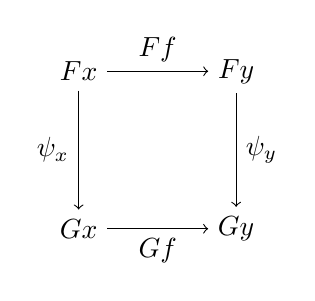
\begin{tikzpicture}
                    \node (FX) at (0, 0) {$Fx$};
                    \node (FY) at(2, 0) {$Fy$};
                    \node (GX) at (0, -2) {$Gx$};
                    \node (GY) at (2, -2) {$Gy$};
                    \draw[->] (FX) -- node[above]{$Ff$} (FY);
                    \draw[->] (GX) -- node[below]{$Gf$} (GY);
                    \draw[->] (FX) -- node[left]{$\psi_x$} (GX);
                    \draw[->] (FY) -- node[right]{$\psi_y$} (GY);
                \end{tikzpicture}
            \end{gather*}
        \end{enumerate}
        It is often said that $\psi_x$ or $\psi$ \textbf{is natural in $x$}.
    }
    \begin{notation}
        A natural transformation $\psi$ from a functor $F$ to a functor $G$ is denoted by $\psi:F\Rightarrow G$.\footnote{This is in analogy with the notation for general 2-morphisms. See section \ref{cat:higher_category_theory} for more information.}
    \end{notation}

    \newdef{Dinatural transformation}{
        Consider two profunctors $\profunc{F,G}{C}{C}$ (this can easily be generalized to functors of the form $F:\mathbf{D}^{op}\times\mathbf{C}\rightarrow\mathbf{E}$). A dinatural transformation is a family of morphisms \[\eta_x:F(x, x)\rightarrow G(x, x)\] that make diagram \ref{fig:dinatural} commute for every morphism $f:y\rightarrow x$.

        \begin{figure}[ht!]
            \centering
            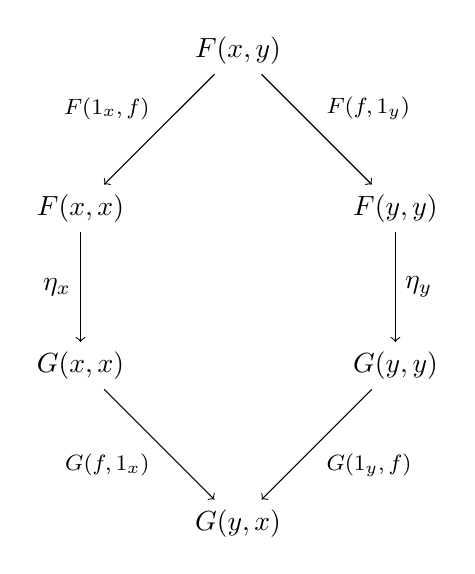
\begin{tikzpicture}
                \node (ab) at (0, 6) {$F(x, y)$};
                \node (F1) at (-2, 4) {$F(x, x)$};
                \node (F2) at (2, 4) {$F(y, y)$};
                \node (G1) at (-2, 2) {$G(x, x)$};
                \node (G2) at (2, 2) {$G(y, y)$};
                \node (ba) at (0, 0) {$G(y, x)$};

                \draw[->] (ab) edge node[above left]{\footnotesize$F(\mathbbm{1}_x, f)$} (F1) (F1) edge node[left]{$\eta_x$} (G1) (G1) edge node[below left]{\footnotesize$G(f, \mathbbm{1}_x)$} (ba);
                \draw[->] (ab) edge node[above right]{\footnotesize$F(f, \mathbbm{1}_y)$} (F2) (F2) edge node[right]{$\eta_y$} (G2) (G2) edge node[below right]{\footnotesize$G(\mathbbm{1}_y, f)$} (ba);
            \end{tikzpicture}
            \caption{Dinatural transformation.}
            \label{fig:dinatural}
        \end{figure}
    }

    \begin{definition}[Functor category]\index{functor!category}
        Consider two categories $\mathbf{C,D}$ where $\mathbf{C}$ is small. The functors $\func{F}{C}{D}$ form the objects of a category with the natural transformations as morphisms. This category is denoted by $\funccat{C}{D}$ or $\mathbf{D}^{\mathbf{C}}$ (the latter is a generalization of \ref{set:function_set}).
    \end{definition}

    \newdef{Representable functor}{\index{functor!representable}
        Let $\mathbf{C}$ be a locally small category. A functor $\func{F}{C}{Set}$ is said to be representable if there exists an object $x\in\ob{C}$ such that $F$ is naturally isomorphic to $h^x$. The pair $(x,\psi)$, where $\psi$ is the natural isomorphism, is called a \textbf{representation} of $F$.
    }
    \remark{A similar definition exists for contravariant functors $G:\mathbf{C}^{op}\rightarrow\mathbf{Set}$. In this case $h^x$ has to be replaced by $h_x$.}

    \begin{theorem}[Yoneda's lemma]\index{Yoneda!lemma}
        Let $\mathbf{C}$ be a locally small category and let $\func{F}{C}{Set}$ be a functor. For every object $x\in\ob{C}$ there exists a natural isomorphism\footnote{Here we use the fact that $\text{Nat}(h^-, -)$ can be seen as a functor $\mathbf{Set}^{\mathbf{C}}\times\mathbf{C}\rightarrow\mathbf{Set}$.} $\eta_x:\text{\emph{Nat}}(h^x, F)\rightarrow Fx$. The image of a natural transformation $\psi\in\text{\emph{Nat}}(h^x, F)$ is given by $\psi_x(\mathbbm{1}_x)$.
    \end{theorem}
    \remark{For contravariant functors $G:\mathbf{C}^{op}\rightarrow\mathbf{Set}$ we obtain a similar statement after replacing $\mathbf{C}(x, -)$ by $\mathbf{C}(-, x)$.}

    \begin{result}[Yoneda embedding]
        When $F$ is another hom-functor $h^y$ we obtain the following result:
        \begin{gather}
            \text{Nat}(h^x, h^y)\cong\mathbf{C}(y, x)
        \end{gather}
        Note that $y$ appears in the first argument on the right-hand side.

        Let $\mathbf{C}(f, -)$ denote the natural transformation corresponding to the morphism $f\in\mathbf{C}(y,x)$. The functor $h^-$ mapping an object $x\in\ob{C}$ to its hom-functor $\mathbf{C}(x, -)$ and a morphism $f\in\mathbf{C}(y, x)$ to the natural transformation $\mathbf{C}(f, -)$ can also be interpreted as a covariant functor $G:\mathbf{C}^{op}\rightarrow\mathbf{Set}^{\mathbf{C}}$. This way we see that Yoneda's lemma gives us a fully faithful functor (i.e. an embedding) $h^-$ from the opposite category $\mathbf{C}^{op}$ to the functor category $\mathbf{Set}^{\mathbf{C}}$.

        As usual all of this can be done for contravariant functors. This gives us an embedding
        \begin{gather}
            \mathcal{Y}:=h_-:\mathbf{C}\hookrightarrow\widehat{\mathbf{C}}
        \end{gather}
        called the Yoneda embedding.
    \end{result}

    \newdef{Local object}{\index{local!object}\label{cat:local_object}
        Consider a collection of morphisms $S\subset\text{hom}(\mathbf{C})$. An object $c\in\ob{C}$ is said to be $S$-local if the Yoneda embedding $\mathcal{Y}c$ maps morphisms in $S$ to isomorphisms in $\mathbf{Set}$. A morphism $f\in\text{hom}(\mathbf{C})$ is said to be $S$-local if its image under the Yoneda embedding of every $S$-local object is an isomorphism in $\mathbf{Set}$.
    }

\subsection{Equivalences}

    \newdef{Equivalence of categories}{\index{equivalence!of categories}
        Two categories $\mathbf{C}, \mathbf{D}$ are said to be equivalent if there exist functors $\func{F}{C}{D}$ and $\func{G}{D}{C}$ such that $FG$ and $GF$ are naturally isomorphic to identity functors.

        A weaker notion is that of a \textbf{weak equivalence}: Two categories $\mathbf{C},\mathbf{D}$ are said to be weakly equivalent if there exists functors $\func{F}{C}{D}$ and $\func{G}{D}{C}$ that are fully faithful and essentially surjective. Assuming the axiom of choice, every weak equivalence is also a strong equivalence (in fact this is equivalent to the axiom of choice).
    }

    \newdef{Skeletal category}{\index{category!skeletal}
        A category in which isomorphic objects are equal, i.e. every isomorphism is an identity morphism. The \textbf{skeleton} of a category is an equivalent skeletal category (often taken to be a subcategory by choosing a representative for every isomorphism class).

        If one does not assume the axiom of choice, the skeleton is merely a \textit{weakly equivalent} skeletal category.
    }

    \newdef{Decategorification}{\index{decategorification}\label{cat:decategorification}
        Let $\mathbf{C}$ be a (essentially) small category. The set of isomorphism classes of $\mathbf{C}$ is called the decategorification of $\mathbf{C}$. This amounts to a functor $\func{\text{Decat}}{Cat}{Set}$. This can also be generalized to higher category theory as a functor $n\mathbf{Cat}\rightarrow(n-1)\mathbf{Cat}$.
    }

\subsection{Stuff, structure and property}\index{forgetful}

    To classify properties of objects and the \textit{forgetfulness} of functors it is interesting to make a distinction between stuff, structure and properties. Consider for example a group: this is a set (\textit{stuff}) equipped with a number of operations (\textit{structure}) that obey some relations (\textit{properties}).

    Using these notions we can classify forgetful functors in the following way:
    \begin{itemize}
        \item A functor forgets nothing if it is an equivalence of categories.
        \item A functor forgets at most properties if it is fully faithful.
        \item A functor forgets at most structure if it is faithful.
        \item A functor forgets at most stuff if it is just a functor.
    \end{itemize}

    ?? COMPLETE (see e.g. nLab or the paper "Why surplus structure is not superfluous" by Nicholas Teh et al.) ??

\subsection{Adjunctions}\index{adjunction}\label{section:adjunction}

    \newdef{Hom-set adjunction}{
        Let $\func{F}{C}{D}$ and $\func{G}{D}{C}$ be two functors. These functors form a hom-set adjunction (often just called an adjunction) if the following isomorphism is natural in both $a$ and $b$:
        \begin{gather}
            \mathbf{D}(Fa, b)\cong\mathbf{C}(a, Gb).
        \end{gather}
        The functor $F$ (resp. G) is called the left (resp. right) adjoint and the image of a morphism under either of the natural isomoprhisms is called the adjunct of the morphism.\footnote{Sometimes the word \textbf{adjunct} is also used instead of adjoint (cf. French versus Latin).}.
    }
    \begin{notation}
        An adjunction $(F,G)$ between categories $\mathbf{C,D}$ is often denoted by \[\mathbf{D}\adj{F}{G}\mathbf{C}\] or, if the ambient categories are clear, by \[F\dashv G.\]
    \end{notation}

    \newdef{Unit-counit adjunction}{\index{triangle!identities}\index{unit}\index{zig-zag|see{triangle identity}}
        Let $\func{F}{C}{D}$ and $\func{G}{D}{C}$ be two functors. These functors form a unit-counit adjunction if there exist natural transformations
        \begin{align}
            \varepsilon: F\circ G\Rightarrow 1_D\\
            \eta: 1_C\Rightarrow G\circ F
        \end{align}
        such that the following compositions are identity morphisms:
        \begin{align}
            F\xrightarrow{F\eta}FGF&\xrightarrow{\varepsilon F}F\\
            G\xrightarrow{\eta G}GFG&\xrightarrow{G\varepsilon}G.
        \end{align}
        These identities are sometimes called the \textbf{triangle} or \textbf{zig-zag identities} (the latter results from the shape of the associated \textit{string diagram}). The transformations $\eta$ and $\varepsilon$ are called the \textbf{unit} and \textbf{counit} respectively.
    }

    \begin{property}[Equivalence of the above definitions]
        Every hom-set adjunction induces a unit-counit adjunction: Let $\Phi_{a,b}$ be the natural isomorphism associated to the hom-set adjunction $F\dashv G$. The unit $\varepsilon_d$ is obtained as the adjunct $\Phi^{-1}_{Gd,d}(\mathbbm{1}_{Gd})$ of the identity morphism on $Gd\in\ob{C}$, and the counit $\eta_c$ is analogously defined as the adjunct $\Phi_{c,Fc}(\mathbbm{1}_{Fc})$ of the identity morphism at $Fc\in\ob{D}$.

        Conversely, every unit-counit adjunction induces a hom-set adjunction: Consider a morphism $f:Fc\rightarrow d$. The (right) adjunct is defined as the composition \[\tilde{f}:=Gf\circ\eta_c:c\rightarrow (G\circ F)c\rightarrow Gd.\] To construct a (left) adjunct we consider a morphism $\tilde{g}:c\rightarrow Gd$: \[g:=\varepsilon_d\circ F\tilde{g}: Fc\rightarrow (F\circ G)d\rightarrow d.\]
    \end{property}

    \newdef{Reflective subcategory}{\index{category!reflective}\label{cat:reflective_inclusion}
        A full subcategory is said to be reflective (resp. coreflective) if the inclusion functor admits a left (resp. right) adjoint.
    }
    \begin{property}[Adjoint equivalence]\index{equivalence!adjoint}
        Any equivalence of categories is part of an ''adjoint equivalence'', i.e. an adjunction for which the unit and counit morphisms are invertible.
    \end{property}

    Now, it should be obvious that the above definition of a unit-counit adjunction can be generalized to general 2-categories\footnote{See section \ref{cat:higher_category_theory} for more information.}:
    \newdef{\difficult{Adjunction in 2-category}}{
        Let $\mathbf{C}$ be a 2-category. An adjunction in $\mathbf{C}$ is a pair of 1-morphisms $F:a\rightarrow b$ and $G:b\rightarrow a$ together with 2-morphisms $\varepsilon:F\circ G\Rightarrow\mathbbm{1}_b$ and $\eta:\mathbbm{1}_a\Rightarrow G\circ F$ that satisfy the zig-zag identities.
    }
    \begin{remark}[Duals and adjunctions]
        If we look at the defining relations of duals in a rigid monoidal category (see section \ref{section:duality} further on), it should be clear that these are in fact the same as the defining relations of the unit and counit of an adjunction. This is a consequence of the fact that a 2-category with a single object can be regarded as a (strict) monoidal category where the composition in the 2-category becomes the tensor product in the monoidal category. Similarly, adjoint 1-morphisms in the 2-category become duals in the monoidal category.
    \end{remark}

\section{General constructions}

    \newdef{Dagger category\footnotemark}{\index{category!dagger}\index{involution}\label{cat:dagger_category}
        \footnotetext{Also called a \textbf{$\dag$-category}.}
        A category equipped with a contravariant endofunctor such that:
        \begin{enumerate}
            \item for all $c\in\ob{C}: \mathbbm{1}_c^\dag = \mathbbm{1}_c$, and
            \item $\dag\circ\dag = \text{id}$.
        \end{enumerate}
        The second property says that $\dag$ is an \textbf{involutive} functor.
    }
    \begin{remark}\index{unitary}\index{self-adjoint}
        The concept of a dagger structure allows the usual definition of \textbf{unitary} and \textbf{self-adjoint} morphisms:
        \begin{gather}
            f^\dagger = f^{-1}\qquad\text{and}\qquad f^\dagger = f.
        \end{gather}
    \end{remark}
    \begin{property}
        The unitary morphisms in a dagger category form a groupoid\footnote{See definition \ref{cat:groupoid} further below.}.
    \end{property}

    \newdef{Comma category}{\index{category!comma}
        Let $\mathbf{A}, \mathbf{B}$ and $\mathbf{C}$ be three categories and let $\func{F}{A}{C}$ and $\func{G}{B}{C}$ be two functors. The comma category $F\downarrow G$ is defined as follows:
        \begin{itemize}
            \item Objects are triples $(a,b,\gamma)$ where $a\in\ob{A},b\in\ob{B}$ and $\gamma:Fa\rightarrow Gb$.
            \item Morphisms $(a,b,\gamma)\rightarrow(k,l,\sigma)$ are pairs $(f,g)$ where $f:a\rightarrow k\in\text{hom}(\mathbf{A})$ and $g:b\rightarrow l\in\text{hom}(\mathbf{B})$ such that $\sigma\circ Ff = Gg\circ\gamma$.
            \item Composition of morphisms is defined componentwise.
        \end{itemize}
    }
    \newdef{Arrow category}{\index{category!arrow}\index{walking!arrow}\index{interval!category}
        The comma category of the pair of functors $(\text{id},\text{id})$. This is equivalently the functor category $[\mathbf{2},\mathbf{C}]$ where $\mathbf{2}$ is the \textbf{interval category/walking arrow} $\{0\rightarrow1\}$.
    }
    \newdef{Functorial factorization}{\index{factorization!functorial}\label{cat:functorial_factorization}
        A \textit{section} of the composition functor \[\func{\circ}{[3,C]}{[2,C]}.\]
    }

    \newdef{Slice category}{\index{category!slice}
        Let $\mathbf{C}$ be a category and let $c\in\ob{C}$. The slice category $\mathbf{C}/c$ of $\mathbf{C}$ over $c$ is defined as follows:
        \begin{itemize}
            \item The objects are morphisms in $\mathbf{C}$ with codomain $c$.
            \item The morphisms $f\rightarrow g$ are morphisms $h$ in $\mathbf{C}$ such that $g\circ h = f$.
        \end{itemize}
        This category is also called the \textbf{over-category} of $c$. By dualizing we obtain the \textbf{under-category} of $c$.
    }

\subsection{\difficult{Fibred categories}}\label{section:fibred_categories}

    \newdef{Fibre category}{\index{fibre!category}\label{cat:fibre_category}
        Let $\func{\Pi}{A}{B}$ be a functor. The fibre category (of $\Pi$) over $b\in\ob{B}$ is the subcategory of $\textbf{A}$ consisting of all objects $a\in\ob{A}$ such that $\Pi a=b$ and all morphisms $m:a\rightarrow a'$ such that $\Pi m=\mathbbm{1}_b$. We will denote it by $\textbf{A}_\textbf{b}$.

        Morphisms in $\mathbf{A}$ that are mapped to a morphism $f$ in $\mathbf{B}$ are called \textbf{$f$-morphisms} and, in particular (using the identification of objects and their identity morphisms), morphisms in $\textbf{A}_\textbf{b}$ are called \textbf{$b$-morphisms}. Similarly, we can define \textbf{$B$-categories} as the categories $\mathbf{A}$ equipped with a (covariant) functor $\func{\Pi}{A}{B}$. It is not hard to see that these form a \textit{2-category} under composition of functors that respects the $\mathbf{B}$-category structure.
    }

    \newdef{Cartesian morphism}{\index{Cartesian!morphism}
        Consider a $\mathbf{B}$-category $\func{\Pi}{A}{B}$. A morphism $f$ in $\mathbf{A}$ is called $\Pi$-Cartesian if every $\Pi f$-morphism factors uniquely through a $b$-morphism, where $b$ is the domain of $\Pi f$.

        There also exists a notion of \textbf{strong Cartesian morphisms}: A strongly Cartesian morphism is a morphism $f$ such that for every morphism $\varphi$ and every factorization of $\Pi\varphi$ through $\Pi f$ there exists a unique factorization of $\varphi$ through $f$ that maps to the given factorization of $\Pi\varphi$. However, for our case of interest (Grothendieck fibrations) these notions coincide.

        To clarify the above (technical) definitions we can draw the following diagram (where the triangles commute):
        \begin{gather*}
            \begin{tikzpicture}
                \node (X3) at (0,2) {$\forall x'$};
                \node (X1) at (0,0) {$x_1$};
                \node (X2) at (2,0) {$x_2$};
                \node (arrow) at (4,1) {$\overset{\Pi}{\mapsto}$};
                \node (pX3) at (6,2) {$\Pi x'$};
                \node (pX1) at (6,0) {$\Pi x_1$};
                \node (pX2) at (8,0) {$\Pi x_2$};
                \draw[->] (X1) -- node[below]{$f$} (X2);
                \draw[->] (X3) -- node[left]{$\exists! f_b$} (X1);
                \draw[->] (X3) -- node[above right]{$\forall\varphi$} (X2);
                \draw[->] (pX1) -- node[below]{$\Pi f$} (pX2);
                \draw[->] (pX3) -- node[left]{$\forall \nu$} (pX1);
                \draw[->] (pX3) -- node[above right]{$\Pi\varphi$} (pX2);
            \end{tikzpicture}
        \end{gather*}
        The diagram for (weak) Cartesian morphisms is obtained by identifying the objects $\Pi x'$ and $\Pi x_1$, i.e. by restricting to the case $\nu=\mathbbm{1}_{\Pi x_1}$.

        The Cartesian morphisms are said to be \textbf{inverse images} of their projections under $\Pi$ and the object $x_1$ is called an \textbf{inverse image} of $x_2$ by $\Pi f$. The Cartesian morphisms of a fibre category are exactly the isomorphisms of that category.
    }

    \newdef{Fibred category}{\index{fibred!category}\index{Grothendieck!fibration|see{fibred category}}\index{fibration}
        A $\mathbf{B}$-category $\func{\Pi}{A}{B}$ is called a fibred category or \textbf{Grothendieck fibration} if the following conditions are satisfied:
        \begin{enumerate}
            \item Each morphism in $\mathbf{B}$ whose codomain lies in the range of $\Pi$ has at least one inverse image (in the weak sense).
            \item The composition of two Cartesian morphisms is again Cartesian (in the weak sense).
        \end{enumerate}
        If we instead work with strongly Cartesian morphisms, the closure under composition follows from the first part of the definition. However, in a fibred category a morphism weakly Cartesian if and only if it is strongly Cartesian.
    }
    \newdef{Cleavage}{\index{cleavage}\index{cloven|see{cleavage}}
        Given a $\mathbf{B}$-category $\func{\Pi}{A}{B}$, a cleavage is the choice of a Cartesian morphism $f:a\rightarrow a'$ for every $a'\in\ob{A}$ and morphism $g:\Pi a\rightarrow \Pi a'$ such that $\Pi f=g$. A $\mathbf{B}$-category equipped with a cleavage is said to be \textbf{cloven}.

        It is clear that the existence of cleavage is sufficient for a category to be fibred and, conversely (assuming the axiom of choice), every fibred category admits a cleavage.
    }

    The following example can be obtained as a Grothendieck fibration for which every fibre is discrete:
    \begin{example}[Discrete fibration]
        A functor $\func{F}{A}{B}$ such that for every object $a\in\ob{A}$ and every morphism $f:b\rightarrow Fa$ in $\mathbf{B}$ there exists a unique morphism $g:c\rightarrow a$ in $\mathbf{A}$ such that $Fg = f$.
    \end{example}
    \begin{example}[Groupoidal fibration]
        If we require that every morphism in $E$ is Cartesian, we obtain the notion of a groupoid(al) fibration or a \textbf{category fibred in groupoids}. The reason for this name is that every fibre becomes a groupoid. An equivalent definition is that the associated pseudofunctor (see the construction below) factors through the embedding $\mathbf{Grpd}\hookrightarrow\mathbf{Cat}$.
    \end{example}

    \begin{property}[\difficult{Grothendieck construction}]\index{Grothendieck!construction}
        Every cloven category $\func{\Pi}{A}{B}$ defines a \textit{pseudofunctor}\footnote{See definition \ref{cat:pseudofunctor} towards the end of this chapter.} $\cfunc{F}{B}{Cat}$ which sends objects to fibre categories and arrows $f:b\rightarrow b'$ to the pullback functor $f^*$ constructed from a Cartesian morphism covering $f$.

        Conversely, every pseudofunctor gives rise to a fibred category through what is called the \textit{Grothendieck construction}. Furthermore, these two constructions constitute a (2-)equivalence of (2-)categories.

        ?? MAYBE ADD THE Grothendieck construction ??
    \end{property}
    \begin{property}[Functors]\index{split}
        A pseudofunctor is a functor if and only if the cleavage of the associated fibred category is \textbf{splitting}, i.e. it contains all identities and is closed under composition.
    \end{property}

\subsection{Monads}

    \newdef{Monad}{\index{monad}\label{cat:monad}
        A monad is a triple $(T,\mu,\eta)$ where $\func{T}{C}{C}$ is an endofunctor and $\mu:T^2\rightarrow T, \eta:\text{id}_{\mathbf{C}}\rightarrow T$ are natural transformations satisfying the following (coherence) conditions:
        \begin{enumerate}
            \item As natural transformations from $T^3$ to $T$ we have
            \begin{gather}
                \mu\circ T\mu = \mu\circ\mu_T.
            \end{gather}
            \item As natural transformations from $T$ to itself we have
            \begin{gather}
                \mu\circ T\eta = \mu\circ\eta_T = \mathbbm{1}.
            \end{gather}
        \end{enumerate}
        These conditions say that a monad is a monoid \ref{set:monoid} in the category $\mathbf{End}_{\mathbf{C}}$ of endofunctors on $\mathbf{C}$. Accordingly, we often call $\eta$ and $\mu$ the \textbf{unit} and \textbf{multiplication} maps.
    }

    \begin{example}[Adjunction]
        Every adjunction $F\dashv G$, with unit $\varepsilon$ and counit $\eta$, induces a monad of the form $(GF, G\varepsilon F, \eta)$.
    \end{example}

    \newdef{Algebra\footnotemark\ over a monad}{\index{algebra!over a monad}
        \footnotetext{A more suitable name would be ''module over a monad'', since these are modules over a monoid if we regard monads as monoids in $\mathbf{End}_{\mathbf{C}}$.}
        Consider a monad $(T,\mu,\eta)$ on a category $\mathbf{C}$. A algebra over $T$ is a couple $(a,\kappa)$, where $a\in\ob{C}$ and $\kappa:Ta\rightarrow a$, such that the following conditions are satisfied:
        \begin{enumerate}
            \item $\kappa\circ T\kappa = \kappa\circ\mu_a$, and
            \item $\kappa\circ\eta_a = \mathbbm{1}_a$.
        \end{enumerate}
        Morphisms $(a,\kappa_a)\rightarrow(b,\kappa_b)$ of $T$-algebras are morphisms $f:a\rightarrow b$ in $\mathbf{C}$ such that $f\circ\kappa_a = \kappa_b\circ Tf$. An algebra of the form $(Ta,\mu_a)$ is said to be \textbf{free}.
    }
    \newdef{Eilenberg-Moore category}{\index{Eilenberg-Moore category}
        Given a monad $T$ over a category $\mathbf{C}$ we define the Eilenberg-Moore category $\mathbf{C}^T$ as the category of $T$-algebras.
    }
    \newdef{Kleisli category}{\index{Kleisli category}
        Consider a monad $T$ on a category $\mathbf{C}$. The Kleisli category $\mathbf{C}_T$ is the full subcategory of $\mathbf{C}^T$ on the \textbf{free} $T$-algebras. This is equivalently the category with objects $\text{ob}(\mathbf{C}_T):=\ob{C}$ and morphisms $\mathbf{C}_T(a, b):=\mathbf{C}(a, Tb)$.
    }

    \newdef{Monadic adjunction}{\index{adjunction!monadic}
        An adjunction between categories $\mathbf{C}$ and $\mathbf{D}$ is said to be monadic if there exists an equivalence between $D$ and the Eilenberg-Moore category of the induced monad.
    }
    \newdef{Monadic functor}{\index{functor!monadic}
        A functor is said to be monadic if it admits a left adjoint such that the adjunction is monadic.
    }

    The following theorem characterizes monadic functors (for more information on some of the concepts, see section \ref{cat:section:morphisms} further below):
    \begin{theorem}[Beck's monadicity theorem]\index{Beck's monadicity theorem}
        Consider a functor $\func{F}{C}{D}$. This functor is monadic if and only if the following conditions are satisfied:
        \begin{itemize}
            \item $F$ admits a left adjoint.
            \item $F$ reflects isomorphisms.
            \item $\mathbf{C}$ has all coequalizers of $F$-split parallel pairs\footnote{These are parallel pairs $f,g$ such that the images $Ff,Fg$ under $F$ admit a split coequalizer.} and $F$ preserves these coequalizers.
        \end{itemize}
    \end{theorem}
    \remark{A sufficient condition for monadicity is obtained by replacing the third condition above by the following weaker statement: ''$\mathbf{C}$ has all coequalizers of reflexive pairs and $F$ preserves these coequalizers.'' This weaker form is called the \textbf{crude monadicity theorem}.}

    \newdef{Closure operator\footnotemark}{\label{cat:closure_operator}\index{closure!operator}\index{modal operator|see{closure operator}}
        \footnotetext{Also called a \textbf{modal operator}.}
        Consider a monad $(\func{T},\eta,\mu)$. This monad is called a closure operator if the multiplication map is a natural isomorphism.

        Given a closure operator $\func{T}{C}{C}$, we call the object $Tx$ the closure of $x\in\ob{C}$. The morphism $\eta_x$ for $x\in\ob{C}$ is called the \textbf{closing map} and $x$ itself is said to be $T$\textbf{-closed} exactly if its closing map is an isomorphism.
    }

    \begin{remark}[\difficult{Bicategories}]
        In fact we can define a monad in any bicategory as a 1-morphism $t:c\rightarrow c$ together with two 2-morphisms that satisfy similar conditions as the ones above. The above definition is then just a specific case of this more general definition in the 2-category $\mathbf{Cat}$.

        In this general setting we can then also define a \textbf{module} over a monad. First of all we can regard any object $a\in\ob{C}$ as a functor from the terminal category $1$. We can then replace $1$ by any other category in the ordinary definition to obtain a general algebra (or module) over a given monad. It is this definition that readily generalizes to bicategories, i.e. a module is a 1-morphism $a:b\rightarrow c$ together with a 2-morphism that satisfies the same conditions as for an algebra over a monad in $\mathbf{Cat}$.
    \end{remark}

\section{Morphisms and diagrams}\label{cat:section:morphisms}
\subsection{Morphisms}

    \newdef{Section}{\index{section}\index{retract}
        A section of a morphism $f:a\rightarrow b$ is a right-inverse, i.e. a morphism $g:b\rightarrow a$ such that $f\circ g=\mathbbm{1}_b$. $f$ itself is called a \textbf{retraction} of $g$ and $b$ is called a \textbf{retract} of $a$.
    }
    \newdef{Monomorphism}{\index{monomorphism}
        Let $\mathbf{C}$ be a category. A morphism $\mu\in\mathbf{C}(a, b)$ is called a monomorphism, \textbf{mono} or \textbf{monic morphism} if for every object $c\in\ob{C}$ and every two morphisms $\alpha_1, \alpha_2\in\mathbf{C}(c, a)$ such that $\mu\circ\alpha_1 = \mu\circ\alpha_2$ we can conclude that $\alpha_1=\alpha_2$.
    }
    \newdef{Epimorphism}{\index{epimorphism}
        Let $\mathbf{C}$ be a category. A morphism $\varepsilon\in\mathbf{C}(a, b)$ is called an epimorphism, \textbf{epi} or \textbf{epic morphism} if for every object $c\in\ob{C}$ and every two morphisms $\alpha_1, \alpha_2\in\mathbf{C}(b, c)$ such that $\alpha_1\circ\varepsilon = \alpha_2\circ\varepsilon$ we can conclude that $\alpha_1=\alpha_2$.
    }

    \newdef{Split monomorphism}{\index{split}
        A morphism $f:a\rightarrow b$ that is a section of some other morphism $g:b\rightarrow a$. It can be shown that every split mono is in fact a mono and even an \textbf{absolute mono}, i.e. it is preserved by all functors.

        The morphism $g$ can be seen to satisfy the dual condition and hence is called a split epimorphism. Again it can be shown to be an absolute epi.
    }

    \newdef{Balanced category}{\index{category!balanced}\label{category:balanced}
        A category in which every monic epi is an isomorphism.
    }

    \newdef{Reflexive pair}{
        Two parallel morphisms $f,g:a\rightarrow b$ are said to form a reflexive pair if they have a common section, i.e. if there exists a morphism $\sigma:b\rightarrow a$ such that $f\circ\sigma=g\circ\sigma=\mathbbm{1}_b$.
    }

    \newdef{Subobject}{\index{subobject}
        Let $\mathbf{C}$ be a category and let $a\in\ob{C}$ be any object. A subobject $b$ of $a$ is a mono $b\hookrightarrow a$.

        In fact we should work up to isomorphism and, accordingly, the formal definition goes as follows: A subobject $b$ of $a$ in the category $\mathbf{C}$ is an isomorphism class of monos $i:b\hookrightarrow a$ in the slice category $\mathbf{C}/a$.
    }
    \newdef{Well-powered category}{\index{well!powered}
        A category $\mathbf{C}$ is said to be well-powered if for every object $a\in\ob{C}$ the class of subobjects $\text{Sub}(a)$ is small.
    }

\subsection{Initial and terminal objects}

    \newdef{Initial object}{
        An object $\emptyset$ such that for every other object $x$ there exists a unique morphism $\iota_x:\emptyset\rightarrow x$.
    }
    \newdef{Terminal object}{
        An object $1$ such that for every other object $x$ there exists a unique morphism $\tau_x:x\rightarrow 1$.
    }
    \begin{property}[Uniqueness]
        If an initial (resp. terminal) object exists, then it is unique (up to isomorphisms).
    \end{property}

    \newdef{Zero object}{\index{zero!object}\label{cat:zero_object}
        An object that is both initial and terminal. The zero object is often denoted by $0$.
    }
    \begin{property}[Zero morphism]
        From the definition of the zero object it follows that for any two objects $a,b$ there exists a unique morphism $0_{ab}:a\rightarrow0\rightarrow b$.
    \end{property}
    \newdef{Pointed category}{\index{pointed!category}\label{category:pointed_category}
        A category containing a zero object.
    }

    \newdef{Global element}{\index{global!element}\label{category:global_element}
        Let $\mathbf{C}$ be a category with terminal object $1$. A global element of an object $c\in\ob{C}$ is a morphism $1\rightarrow c$.
    }
    \begin{property}
        Every global element is monic.
    \end{property}
    \newdef{Pointed object}{\index{pointed!object}
        An object $c$ equipped with a global element $1\rightarrow c$. (This morphism is sometimes called the \textbf{basepoint}.)
    }

    \begin{remark}\label{cat:global_elements_remark}
        In the category $\mathbf{Set}$ the elements of a set $S$ are in one-to-one correspondence with the global elements of $S$. Furthermore, we have the important property (\textit{axiom of functional extensionality}) that two functions $f,g:S\rightarrow S'$ coincide if their values at every element $s\in S$ coincide or, equivalently, if their precompositions with global elements coincide.

        However, this way of checking equality can fail in other categories. Consider for example $\mathbf{Grp}$, the category of groups, with its zero object $0=\{e\}$. The only morphism from this group to any other group $G$ is the one mapping $e$ to the unit in $G$. It is obvious that precomposition with this morphism tells us nothing about the equality of other morphisms. To recover the extensionality property from $\mathbf{Set}$ we need to generalize the notion of ''element'':
    \end{remark}
    \newdef{Generalized element}{\index{shape}
        Let $\mathbf{C}$ be category and consider an object $c\in\ob{C}$. For any object $y\in\ob{C}$ we call a morphism $b\rightarrow c$ a generalized element of $c$. The morphisms $b\rightarrow c$ are also called \textbf{$b$-elements} in $c$ or elements of \textbf{shape} $b$ in $c$.
    }

    \newdef{Generator}{\index{generator}\index{separator|see{generator}}\label{cat:generator}
        Let $\mathbf{C}$ be a category. A collection of objects $\mathcal{O}\subset\ob{C}$ is called a collection of generators or \textbf{separators} for $\mathbf{C}$ if, given any two objects $a,b\in\ob{C}$ and any two parallel morphisms $f,g:a\rightarrow b$, we have that
        \begin{gather}
            f\neq g\implies\exists o\in\mathcal{O},\exists h\in\mathbf{C}(o, a): f\circ h\neq g\circ h.
        \end{gather}
        Equivalently this says that the generalized elements of the objects in $\mathcal{O}$ are sufficient to distinguish between all morphisms in $\mathbf{C}$.
    }
    \newdef{Well-pointed category}{\index{well!pointed}
        A category for which the terminal object is a generator.
    }

\subsection{Lifts}

    \newdef{Lifts and extensions}{\index{lift}\index{extension}
        A lift of a morphism $f:a\rightarrow b$ along an epi $e:x\rightarrow b$ is a morphism $g:a\rightarrow x$ satisfying $f=e\circ g$. Dualizing this definition gives the notion of extensions. (The epi/mono condition is often dropped in the literature.)
    }
    \newdef{Lifting property}{\index{orthogonal!lifting}\label{cat:lifting_property}
        A morphism $f:a\rightarrow b$ has the left lifting property with respect to a morphism $g:c\rightarrow d$ if for every commutative diagram
        \begin{gather*}
            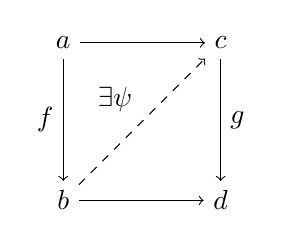
\begin{tikzpicture}
                \node (A) at (0, 0) {$a$};
                \node (B) at (0, -2) {$b$};
                \node (C) at (2, 0) {$c$};
                \node (D) at (2, -2) {$d$};
                \draw[->] (A) -- node[left]{$f$} (B);
                \draw[->] (A) -- (C);
                \draw[->, dashed] (B) -- node[above left]{$\exists\psi$} (C);
                \draw[->] (B) -- (D);
                \draw[->] (C) -- node[right]{$g$} (D);
            \end{tikzpicture}
        \end{gather*}
        there exists a morphism $\psi:b\rightarrow c$ such that the triangles commute. The morphism $g$ is also said to have the right lifting property with respect to $f$. If the morphism $\psi$ is unique, then $f$ and $g$ are said to be \textbf{orthogonal}.
    }
    \newdef{Injective and projective morphisms}{\index{injective!morphism}\index{projective!morphism}
        Consider a class of morphisms $I\subseteq\text{hom}(\mathbf{C})$. A morphism $f\in\text{hom}(\mathbf{C})$ is said to be $I$-injective (resp. $I$-projective) if it has the right (resp. left) lifting property with respect to all morphisms in $I$.

        Given a set of morphisms $I$, we denote the set of $I$-injective morphisms by $\text{rlp}(I)$ and the set of $I$-projective morphisms by $\text{llp}(I)$.
    }
    \newdef{Injective and projective objects}{\index{injective!object}\index{projective!object}
        If $\mathbf{C}$ has a terminal object $1$, an object $x$ is called $I$-injective if its terminal morphism is $I$-injective. If $\mathbf{C}$ has an initial object, we can dually define $I$-projective objects:

        \begin{figure}[ht!]
            \centering
            \begin{subfigure}[b]{0.49\textwidth}
                \centering
                \begin{tikzpicture}
                    \node (A) at (0, 0) {$a$};
                    \node (B) at (0, -2) {$b$};
                    \node (C) at (2, 0) {$i$};
                    \draw[->] (A) -- node[left]{$\forall f\in I$} (B);
                    \draw[->] (A) -- node[above]{$g$} (C);
                    \draw[dashed, ->] (B) -- node[below right]{$\exists\psi$} (C);
                \end{tikzpicture}
                \caption{Injective object $i$.}
                \label{fig:injective_object}
            \end{subfigure}
            \begin{subfigure}[b]{0.49\textwidth}
                \centering
                \begin{tikzpicture}
                    \node (A) at (2, 2) {$a$};
                    \node (B) at (2, 0) {$b$};
                    \node (C) at (0, 0) {$p$};
                    \draw[->] (A) -- node[right]{$\forall f\in I$} (B);
                    \draw[->] (C) -- node[below]{$g$} (B);
                    \draw[dashed, ->] (C) -- node[above left]{$\exists\psi$} (A);
                \end{tikzpicture}
                \caption{Projective object $p$.}
                \label{fig:projective_object}
            \end{subfigure}
        \end{figure}
        In general we speak of \textbf{injective} (resp. \textbf{projective}) objects if $I$ is the class of monomorphisms (resp. epimorphisms). For projective objects this is equivalent to requiring that the (covariant) hom-functor preserves epimorphisms.

        A category $\mathbf{C}$ is said to \textbf{have enough injectives} if for every object there exists a monomorphism into an injective object. The category is said to \textbf{have enough projectives} if for every object there exists an epimorphism from a projective object onto it.
    }
    \newdef{Fibrations and cofibrations}{\index{fibration}
        Consider a category $\mathbf{C}$ together with a class $I\subseteq\text{hom}(\mathbf{C})$ of morphisms. A morphism $f\in\text{hom}(\mathbf{C})$ is called a $I$-fibration (resp. $I$-cofibration) if it has the right (resp. left) lifting property with respect to all $I$-projective (resp. $I$-injective) morphisms.
    }

\subsection{Limits and colimits}\label{section:diagrams}

    \newdef{Diagram}{\index{diagram}
        A diagram in $\mathbf{C}$ with index category $\mathbf{I}$ is a (covariant) functor $\func{D}{I}{C}$.
    }

    \newdef{Cone}{\index{cone}
        Let $\func{D}{I}{C}$ be a diagram. A cone from $a\in\ob{C}$ to $D$ consists of a family of morphisms $\psi_i:a\rightarrow Di$ indexed by $\mathbf{I}$ such that $\psi_j = Df\circ\psi_i$ for all morphisms $f:i\rightarrow j\in\text{hom}(\mathbf{I})$. This is depicted in figure \ref{fig:cone_component}.

        \begin{figure}[ht!]
            \centering
            \begin{subfigure}[b]{0.49\textwidth}
                \centering
                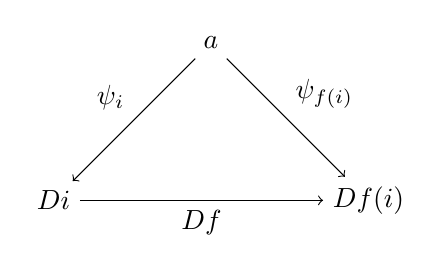
\begin{tikzpicture}
                    \node (1) at (0, 0) {$a$};
                    \node (2) at (-2, -2) {$Di$};
                    \node (3) at (2, -2) {$Df(i)$};
                    \draw[->] (1) -- node[above left]{$\psi_i$} (2);
                    \draw[->] (1) -- node[above right]{$\psi_{f(i)}$} (3);
                    \draw[->] (2) -- node[below]{$Df$} (3);
                \end{tikzpicture}
                \caption{Component of cone over $D$.}
                \label{fig:cone_component}
            \end{subfigure}
            \begin{subfigure}[b]{0.49\textwidth}
                \centering
                \begin{tikzpicture}
                    \node (1) at (0, -2) {$Di$};
                    \node (2) at (-2, 0) {$a$};
                    \node (3) at (2, 0) {$b$};
                    \draw[<-] (1) -- node[below left]{$\psi_i$} (2);
                    \draw[<-] (1) -- node[below right]{$\phi_i$} (3);
                    \draw[->] (2) -- node[above]{$f$} (3);
                \end{tikzpicture}
                \caption{Morphism of cones.}
                \label{fig:cone_morphism}
            \end{subfigure}
            \caption{Category of cones.}
            \label{fig:cone}
        \end{figure}
    }
    \begin{adefinition}\index{diagonal!functor}
        The above definition can be reformulated by defining an additional functor\footnote{The notation $\Delta_a$ tells us that $\Delta:C\rightarrow [\mathbf{I},\mathbf{C}]$ is the \textbf{diagonal functor}, i.e. $\Delta_c\equiv\Delta(c)$ is the constant functor from $\mathbf{I}$ to $\mathbf{C}$ with target object $c$.} $\Delta_a:\mathbf{I}\rightarrow\mathbf{C}$ that maps every element $i\in\ob{I}$ to $a$ and every morphism $g\in\text{hom}(\mathbf{I})$ to $\mathbbm{1}_a$. The morphisms $\psi_i$ can then be seen as the components of a natural transformation $\psi:\Delta_a\Rightarrow D$. Hence a cone $(a,\psi)$ is an element of $[\mathbf{I}, \mathbf{C}](\Delta_a, D)$.
    \end{adefinition}
    \newdef{Morphism of cones}{\index{morphism!of cones}
        Let $\func{D}{I}{C}$ be a diagram and let $(a,\psi)$ and $(b,\phi)$ be two cones over $D$. A morphism between these cones is a morphism of the apexes $f:a\rightarrow b$ such that the diagrams of the form \ref{fig:cone_morphism} commute for all $i\in\ob{I}$. The cones over $D$ together with these morphisms form a category $\mathbf{Cone}(D)$, in fact this can easily be seen to be the comma category $\Delta\downarrow D$.
    }

    \newdef{Limit}{\index{limit}
        Consider a diagram $\func{D}{I}{C}$. The limit of this diagram, denoted by $\lim D$, is (if it exists) the terminal object of the category $\mathbf{Cone}(D)$.
    }
    \begin{remark*}\index{projective!limit}\index{inductive!limit}
        In the older literature the name \textbf{projective limit} was sometimes used. The dual notion, a \textbf{colimit}, is often called an \textbf{inductive limit} in the older literature.
    \end{remark*}
    This definition gives us the following universal property:
    \begin{uproperty}\label{cat:limit_uproperty}
        Let $\func{D}{I}{C}$ be a diagram. For every cone $(c,\psi)\in\mathbf{Cone}(D)$ there exists a unique morphism $f:c\rightarrow\lim D$. This defines a bijection \[[\mathbf{I}, \mathbf{C}](\Delta_c, D) \cong \mathbf{C}(c, \lim D).\]
        If all (small) limits exist, we can define the limit functor $\func{\lim}{[I, C]}{C}$. The universal property of limits then implies that it is right adjoint to the constant functor $\Delta$.

        For diagrams in $\mathbf{Set}$ we can use the fully faithfulness of the Yoneda embedding to obtain the following expression:
        \begin{gather}
            \lim D \cong \funccat{I}{Set}(\Delta_\ast, D).
        \end{gather}
    \end{uproperty}
    \begin{remark}
        In section \ref{section:enriched_category_theory} on enriched category theory we will give a generalization (the so-called \textit{weighted limits}) of the above construction that is better suited to the enriched setting and allows us to express a wide variety of constructions as (weighted) limits.
    \end{remark}

    \begin{example}[Terminal object]
        The terminal object $1$ is the limit over the empty diagram.
    \end{example}

    \newdef{Finitely complete category}{\index{category!complete}
        A category is said to be finitely complete if it has all finite limits. If all (small) limits exist, the category is said to be \textbf{complete}. The dual notion for colimits is called \textbf{(finite) cocompleteness}.
    }
    \begin{example}[Presheaf categories]\label{cat:complete_presheaf_category}
        All presheaf categories are both complete and cocomplete.
    \end{example}

    \newdef{Continuous functor}{\index{continuity!functor}\label{cat:continuity}
        A functor that preserves all small limits.
    }
    \begin{example}[Hom-functors]
        In a locally small category every hom-functor is continuous (in fact these functors even preserve limits that are not necessarily small). This implies for example that
        \begin{gather}
            \mathbf{C}(c, \lim D) \cong \lim\mathbf{C}(c, D).
        \end{gather}
    \end{example}

    In the case where $\mathbf{C}$ is small, we can characterize the Yoneda embedding through a universal property:
    \begin{uproperty}[Free cocompletion]\index{co-!completion}\index{Yoneda!embedding}\label{cat:free_cocompletion}
        The Yoneda embedding $\mathbf{C}\hookrightarrow\widehat{\mathbf{C}}$ turns the presheaf category $\widehat{\mathbf{C}}$ into the \textbf{free cocompletion} of $\mathbf{C}$, i.e. there exists an equivalence of categories between the functor category of cocontinuous functors $[\widehat{\mathbf{C}}, \mathbf{D}]_{\text{cont}}$ and the ordinary functor category $[\mathbf{C}, \mathbf{D}]$.
    \end{uproperty}

    \newdef{Tiny object}{\index{tiny}\label{cat:tiny}
        An object in a locally small category such that its covariant hom-functor preserves small colimits. This is sometimes called a \textbf{small-projective} object since it is in particular projective\footnote{Epimorphisms are characterized by a \textit{pushout} (see definition \ref{cat:pushout_epi} further below).}.
    }
    \newdef{Cauchy completion}{\index{Cauchy!completion}\index{Karoubi!envelope}
        Let $\mathbf{C}$ be a small category. An important (small and full) subcategory of the free cocompletion of $\mathbf{C}$ is given by the Cauchy completion, i.e. the subcategory of $\widehat{\mathbf{C}}$ on the tiny objects.\footnote{A generalization in the context of enriched categories is given by the \textit{Karoubi envelope}.} It can be shown that the free cocompletion of the Cauchy completion coincides with the one on $\mathbf{C}$ (up to equivalence).

        A category is said to be \textbf{Cauchy-complete} if it is equivalent to its Cauchy completion. It can be shown that a category is Cauchy-complete if and only if it has all small absolute colimits.
    }

    \newdef{Filtered category}{\index{category!filtered}
        A category in which every finite diagram admits a cocone. For regular cardinals $\kappa$ we can generalize this notion: A  category is said to be $\kappa$-filtered if every diagram with less than $\kappa$ arrows admits a cocone. (In this terminology filtered categories are the same as $\omega$-filtered categories.)
    }

    \newdef{Directed limit}{\index{limit!directed}
        Consider a diagram $\func{D}{I}{C}$. The limit (resp. colimit) of $D$ is said to be codirected (resp. directed) if $\mathbf{I}$ is a downward (resp. upward) directed set \ref{set:directed_set}.
    }
    The following definition is a categorification of the previous one:
    \newdef{Filtered limit}{\index{limit!filtered}
        Consider a diagram $\func{D}{I}{C}$. The limit (resp. colimit) of $D$ is said to be cofiltered (resp. filtered) if $\mathbf{I}$ is a cofiltered (resp. filtered) category.
    }
    \newdef{Pro-object}{\index{pro!object}
        A functor $\func{F}{I}{C}$ where $\mathbf{I}$ is a small cofiltered category. The names stems from the fact that we can interpet pro-objects as formal cofiltered (projective) limits.
    }

    \begin{property}\label{cat:directed_filtered}
        A category has all directed colimits if and only if it has all filtered colimits. (A dual statement holds for limits.)
    \end{property}

    \newdef{Compact object}{\index{compact}\index{presentable}
        An object for which the covariant hom-functor preserves all filtered colimits. These objects are also said to be \textbf{finitely presentable}.\footnote{This name derives from the fact that modules are finitely presented if and only if their covariant hom-functor preserves direct limits (i.e. directed colimits in the context of algebra).}
    }

    \newdef{Product}{\index{product}\index{co-!product}
        Let $\mathbf{I}$ be a discrete category. The (co)limit over a diagram $\func{D}{I}{C}$ is called a (co)product in $\mathbf{C}$.
    }

    \newdef{Equalizer}{\index{equalizer}\index{fork}
        Consider a diagram of the form \[x\overset{f}{\underset{g}{\rightrightarrows}} y.\] The limit of this diagram is called the equalizer of $f$ and $g$. It consists of an object $e$ and a morphism $\varepsilon:e\rightarrow x$ such that the following \textbf{fork} diagram
        \begin{gather}
            e\xrightarrow{\varepsilon}x\overset{f}{\underset{g}{\rightrightarrows}} y
        \end{gather}
        is universal with respect to $(e,\varepsilon)$. By dualizing we obtain \textbf{cofork} diagrams $x\rightrightarrows y\rightarrow z$ and their universal versions, the \textbf{coequalizers}.
    }
    \newdef{Split coequalizer}{\index{split}\label{cat:split_coequalizer}
        A cofork together with a section $\varphi$ of $f$ and a section $\sigma$ of $\tau$ such that $\sigma\circ\tau = g\circ\varphi$.
    }

    \newdef{Regular morphisms}{\index{regular!morphism}
        A mono (resp. epi) is said to be regular if it arises as an equalizer (resp. coequalizer) of two parallel morphisms.
    }
    \begin{property}[Regular bimorphism]\label{category:regular_iso}
        Both monic regular epimorphisms and epic regular monomorphisms are isomorphisms.
    \end{property}

    \newadef{Finitely complete category}{\index{category!complete}
        A category is said to be finitely complete if it has a terminal object and if all binary equalizers and products exist.
    }

    \newdef{Span}{\index{span}
        A span in a category $C$ is a diagram of the form \ref{fig:cat_span}. Let $\mathbf{\Lambda}$ be the category with three objects $\{-1, 0, 1\}$ and two morphisms $i:0\rightarrow -1$ and $j:0\rightarrow 1$. By the above definition of a diagram, a span in $C$ is equivalent to a functor $\func{S}{\Lambda}{C}$ (therefore we can also call $\Lambda$ the universal span).

        \begin{figure}[!ht]
            \centering
            \begin{subfigure}[b]{0.49\textwidth}
                \centering
                \begin{tikzpicture}
                    \node (A) at (-2, 0) {$a$};
                    \node (S) at (0, 2) {$s$};
                    \node (B) at (2, 0) {$b$};
                    \draw[->] (S) -- node[above left]{$f$} (A);
                    \draw[->] (S) -- node[above right]{$g$} (B);
                \end{tikzpicture}
                \caption{Span (category theory).}
                \label{fig:cat_span}
            \end{subfigure}
            \begin{subfigure}[b]{0.49\textwidth}
                \centering
                \begin{tikzpicture}
                    \node (A) at (-2, 2) {$a$};
                    \node (S) at (0, 0) {$c$};
                    \node (B) at (2, 2) {$b$};
                    \draw[<-] (S) -- node[below left]{$f$} (A);
                    \draw[<-] (S) -- node[below right]{$g$} (B);
                \end{tikzpicture}
                \caption{Cospan.}
                \label{fig:pullback}
            \end{subfigure}
            \caption{}
        \end{figure}
    }

    \newdef{Pullback}{\index{pullback}\index{fibre!product|seealso{pullback}}\index{Cartesian!square}\label{cat:pullback}
        The pullback or \textbf{fibre product} of two morphisms $f:a\rightarrow c$ and $g:b\rightarrow c$ is defined as the limit of cospan \ref{fig:pullback}. The full diagram characterizing the pullback, which has the form of a square, is sometimes called a \textbf{Cartesian square}.
    }
    \begin{notation}[Pullback]
        The pullback of two morphisms $f:a\rightarrow c$ and $g:b\rightarrow c$ is often denoted by $a\times_c b$.
    \end{notation}

    \begin{property}[Product]\index{product}
        If a terminal object $1$ exists, the pullback $a\times_1b$ is equal to the (Cartesian) product $a\times b$.
    \end{property}
    \newdef{Kernel pair}{\index{kernel}
        Consider a morphism $f:a\rightarrow b$. Its kernel pair is defined as the pullback of $f$ along itself.
    }

    \newdef{Pushout}{\index{pushout}
        The dual notion of a pullback, i.e. the colimit of a span.
    }

    \begin{property}
        Pullbacks preserve monos and pushouts preserve epis.
    \end{property}
    \newadef{Epimorphism}{\index{epimorphism}\label{cat:pushout_epi}
        A morphism such that its pushout along itself is the identity.
    }

    \begin{property}[Span category]\label{cat:span_category}
        \nomenclature[S_span]{$\mathbf{Span}(\mathbf{C})$}{span category over $\mathbf{C}$}
        Consider a category $\mathbf{C}$ with pullbacks. The category $\mathbf{Span}(\mathbf{C})$ is defined as the category with the same objects as $\mathbf{C}$ but with spans as morphisms. Composition of spans is given by pullbacks. By including morphisms of spans, we can refine $\mathbf{Span}(\mathbf{C})$ to a bicategory.
    \end{property}

    \newdef{Wedge}{\index{wedge}
        Consider a profunctor $\profunc{F}{C}{C}$. A wedge $e:w\rightarrow F$ is an object $w\in\ob{Set}$ together with a collection of morphisms $e_c:w\rightarrow F(c, c)$ indexed by $\mathbf{C}$ such that for every morphism $f:c\rightarrow c'$ the following diagram commutes:
        \begin{gather*}
            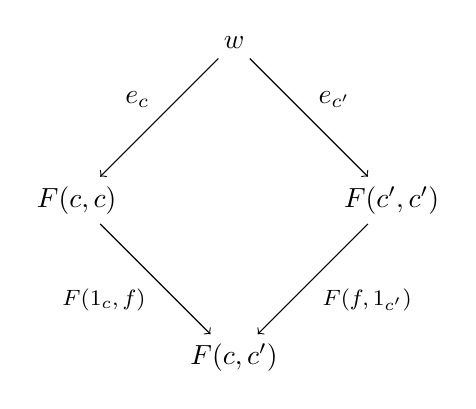
\begin{tikzpicture}
                \node (W) at (0, 4) {$w$};
                \node (F1) at (-2, 2) {$F(c, c)$};
                \node (F2) at (2, 2) {$F(c', c')$};
                \node (F) at (0, 0) {$F(c, c')$};
                \draw[->] (W) edge node[above left]{$e_c$} (F1) (F1) edge node[below left]{\footnotesize$F(\mathbbm{1}_c, f)$} (F);
                \draw[->] (W) edge node[above right]{$e_{c'}$} (F2) (F2) edge node[below right]{\footnotesize$F(f, \mathbbm{1}_{c'})$} (F);
            \end{tikzpicture}
        \end{gather*}
        As was the case for cones, we can reformulate this in terms of (di)natural transformations. A wedge $(w, e)$ of a profunctor $\profunc{F}{C}{C}$ is a dinatural transformation from the constant profunctor $\Delta_w$ to $F$.
    }
    \newdef{End}{\index{end}
        The end of a profunctor $\profunc{F}{C}{C}$ is defined as the universal wedge of $F$. The components of the wedge are called the \textbf{projection maps} of the end. This stems from the fact that for a discrete category the end coincides with the product $\prod_{c\in\ob{C}}F(c, c)$.

        This is equivalent to a definition in terms of equalizers: Consider the two canonical maps $\prod_{c\in\ob{C}}\mathbf{C}(c, c)\rightrightarrows\prod_{f:c\rightarrow c'}\mathbf{C}(c, c')$. This diagram can be interpreted as the product of all lower halves of the wedge diagrams above. It is not hard to see that its equalizer (universally) satisfies the wedge condition for all $f\in\text{hom}(\mathbf{C})$.
    }
    \newnot{End}{
        The end of a profunctor $\profunc{F}{C}{C}$ is often denoted using an integral sign with subscript: \[\int_{c\in\mathbf{C}}F(c, c).\] For the dual construction, called a \textbf{coend}, we use an integral sign with superscript.
    }
    \begin{example}[Natural transformations]\index{natural!transformation}
        Consider two functors $\func{F,G}{C}{D}$. The map $(c,c')\mapsto\mathbf{D}(Fc, Gc')$ gives a profunctor $\profunc{H}{C}{C}$. If we look at the wedge condition for this profunctor (especially the lower half) we get the following equality for all morphisms $f:c\rightarrow c'$:
        \begin{gather}
            \tau_{c'}\circ Ff = Gf\circ \tau_c
        \end{gather}
        where $\tau_c$ is the projection of the wedge associated to the object $c\in\ob{C}$. Comparing this equality to definition \ref{cat:natural} we immediately see that
        \begin{gather}
            \label{cat:natural_end}
            \text{Nat}(F, G) = \int_{c\in\mathbf{C}}\mathbf{D}(Fc, Gc).
        \end{gather}
    \end{example}

    \begin{property}
        Using the continuity \ref{cat:continuity} of the hom-functor we can prove the following equality which can be used to turn ends into coends and vice versa:
        \begin{gather}
            \mathbf{Set}\left(\int^{c\in\mathbf{C}}F(c, c), c'\right) = \int_{c\in\mathbf{C}}\mathbf{Set}\left(F(c, c), c'\right).
        \end{gather}
    \end{property}

    Using the above properties and definitions we obtain the following two statements, called the \textbf{Yoneda reduction} and \textbf{co-Yoneda lemma}:
    \begin{property}[Ninja Yoneda lemma]\index{Yoneda!lemma}\label{cat:ninja_yoneda}
        Let $\func{F}{C}{D}$ be a covariant functor (similar statements hold for contravariant functors).
        \begin{align}
            &\int_{c\in\mathbf{C}}\mathbf{Set}\left(\mathbf{C}(-, c), Fc\right)\cong F\\
            &\int^{c\in\mathbf{C}}\mathbf{C}(c, -)\times Fc\cong F.
        \end{align}
        For a generalization to the enriched setting see definition \ref{cat:enriched_kan_extension}.
    \end{property}
    \begin{remark}
        A common remark at this point is the comparison with the Dirac distribution \ref{distribution:sieving_dirac_delta}:
        \begin{gather}
            \int \delta(x-y)f(x) = f(y).
        \end{gather}
        By interpreting the functor $F$ as a function, we see that the representable functors behave as Dirac distributions.
    \end{remark}

    \newdef{Kan extension}{\index{Kan!extension}\label{cat:kan_extension}
        Consider two functors $\func{F}{C}{D}$ and $\func{G}{C}{E}$. The right Kan extension of $F$ along $G$ is given by the universal functor $\func{\text{Ran}_GF}{E}{D}$ and natural transformation $\eta:\text{Ran}_GF\circ G\Rightarrow F$:
        \begin{gather*}
            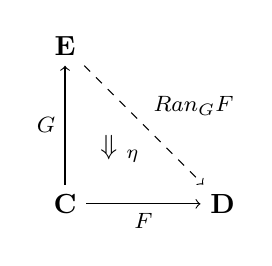
\begin{tikzpicture}
                \node (E) at (0, 2) {$\mathbf{E}$};
                \node (C) at (0, 0) {$\mathbf{C}$};
                \node (D) at (2, 0) {$\mathbf{D}$};
                \node (A) at (0.7, 0.7) {$\Downarrow_{\ \eta}$};
                \draw[->] (C) -- node[left]{\footnotesize$G$} (E);
                \draw[->] (C) -- node[below]{\footnotesize$F$} (D);
                \draw[dashed, ->] (E) -- node[above right]{\footnotesize$\text{Ran}_GF$} (D);
            \end{tikzpicture}
        \end{gather*}
        The left Kan extension $\text{Lan}_GF$ is obtained by dualizing this construction.
    }

    \begin{property}[Complete categories]
        Complete (resp. cocomplete) categories admit all right (resp. left) Kan extensions.
    \end{property}

    \newdef{Absolute Kan extension}{
        A (left\footnote{A analogous definition exists for right Kan extensions.}) Kan extension $\text{Lan}_GF$ is said to be absolute if for every functor $H$ with the same codomain as $F$ the following isomorphism holds:
        \begin{gather}
            H(\text{Lan}_GF)\cong\text{Lan}_G(HF),
        \end{gather}
        i.e. a Kan extension is absolute if right whiskering it by another functor defines the Kan extension of the composition.
    }
    \newdef{Pointwise Kan extension}{\label{cat:pointwise_kan_extension}
        A Kan extension is said to be pointwise if it is preserved by all representable functors.
    }

    \newadef{Kan extension}{
        The construction above gives a functor $\text{Ran}_G$ from the functor category $\funccat{C}{D}$ to the functor category $\funccat{E}{D}$. The right Kan extension $\text{Ran}_G$ can be defined as the right adjoint to the pullback functor $G^*:F\mapsto F\circ G$. Similarly, we can define the left Kan extension as the left adjoint to the pullback functor $G^*$.

        In the spirit of partial adjoints we can use this definition to define \textbf{local Kan extensions}: Although the left (or right) Kan extension functors do not have to exists globally, the extension of a single functor could still exist. This local version is defined by the following natural isomorphism (here given for a left extension):
        \begin{gather}
            \funccat{C}{D}(F, G^*-) \cong \funccat{E}{D}(\text{Lan}_GF, -).
        \end{gather}
    }
    \remark{Using this equivalence of hom-spaces we can generalize the Kan extension from $\mathbf{Cat}$ to any \textit{2-category}.}

    \begin{example}[Limit]\index{limit}
        Denote the terminal category by $\mathbf{1}$. By choosing the functor $G$ in the definition of a right Kan extension to be the unique functor $!_{\mathbf{C}}:\mathbf{C}\rightarrow\mathbf{1}$ we obtain the universal property characterizing limits \ref{cat:limit_uproperty}. We conclude that $\lim F \cong \text{Ran}_{!_C}F$. Similarly, we can obtain the colimit as the left Kan extension.
    \end{example}

    The existence of Kan extensions can also be used to determine the existence of adjoints:
    \begin{property}[Adjoint functors]
        A functor $\func{F}{C}{D}$ admits a left (resp. right) adjoint if and only if the right (resp. left) Kan extension of the identity functor $\func{\mathbbm{1}}{C}{C}$ along $F$ exists. If it exists and if it is an absolute extension, the left adjoint is given exactly by this Kan extension.
    \end{property}

    \newdef{Codensity monad}{\index{monad!codensity}\index{co-!dense}
        Consider a general functor $\func{F}{C}{D}$. If the right Kan extension $\text{Ran}_FF$ exists, then it defines a monad. Functors for which this monad is the identity are said to be \textbf{codense}.\footnote{Codense functors are usually defined in a different way, but we can show that this is an equivalent definition (hence the name).} Left Kan extensions give by duality rise to \textit{density comonads}.
    }

\section{Monoidal categories}

    \newdef{Monoidal category}{\index{monoidal!category}\index{tensor!product}\label{category:monoidal_category}
        A category $\mathbf{C}$ equipped with a bifunctor \[-\otimes -:\mathbf{C}\times\mathbf{C}\rightarrow\mathbf{C}\] called the \textbf{tensor product} or \textbf{monoidal product}, a distinct object $\mathbf{1}$ called the \textbf{unit object}, and the following 3 natural isomorphisms called the \textbf{coherence maps}:
        \begin{enumerate}
            \item \textbf{Associator}: $\alpha_{a, b, c}:(a\otimes b)\otimes c\cong a\otimes(b\otimes c)$,
            \item \textbf{Left unitor}: $\lambda_a:\mathbf{1}\otimes a\cong a$, and
            \item \textbf{Right unitor}: $\rho_a:a\otimes\mathbf{1}\cong a$
        \end{enumerate}
        These natural transformations are required make the \textbf{triangle} and \textbf{pentagon} diagrams commute. (See figures \ref{fig:triangle_diagram} and \ref{fig:pentagon_diagram}.)

        \begin{figure}[ht!]
            \centering
            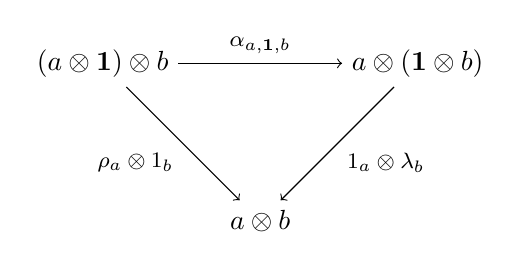
\begin{tikzpicture}
                \node (1) at (0, 0) {$(a\otimes\mathbf{1})\otimes b$};
                \node (2) at (4, 0) {$a\otimes(\mathbf{1}\otimes b)$};
                \node (3) at (2, -2) {$a\otimes b$};
                \draw[->] (1) -- node[above]{\footnotesize$\alpha_{a, \mathbf{1}, b}$} (2);
                \draw[->] (1) -- node[below left]{\footnotesize$\rho_a\otimes\mathbbm{1}_b$} (3);
                \draw[->] (2) -- node[below right]{\footnotesize$\mathbbm{1}_a\otimes\lambda_b$} (3);
            \end{tikzpicture}
            \caption{Triangle diagram.}
            \label{fig:triangle_diagram}
        \end{figure}
        \begin{figure}[ht!]
            \centering
            \begin{tikzpicture}
                \node (1) at (0, 0) {$((a\otimes b)\otimes c)\otimes d$};
                \node (2) at (6, 0) {$(a\otimes (b\otimes c))\otimes d$};
                \node (3) at (-3, -3) {$(a\otimes b)\otimes(c\otimes d)$};
                \node (4) at (9, -3) {$a\otimes((b\otimes c)\otimes d)$};
                \node (5) at (3, -6) {$a\otimes(b\otimes (c\otimes d))$};
                \draw[->] (1) -- node[above]{\footnotesize$\alpha_{a, b, c}\otimes\mathbbm{1}_d$} (2);
                \draw[->] (1) -- node[above left]{\footnotesize$\alpha_{a\otimes b, c, d}$} (3);
                \draw[->] (3) -- node[below left]{\footnotesize$\alpha_{a, b, c\otimes d}$} (5);
                \draw[->] (2) -- node[above right]{\footnotesize$\alpha_{a, b\otimes c, d}$} (4);
                \draw[->] (4) -- node[below right]{\footnotesize$\mathbbm{1}_a\otimes\alpha_{b, c, d}$} (5);
            \end{tikzpicture}
            \caption{Pentagon diagram.}
            \label{fig:pentagon_diagram}
        \end{figure}
    }

    \newdef{Strict monoidal category}{
        A monoidal category for which the associator $\alpha$ and the unitors $\lambda,\rho$ are identity transformations.
    }

    \newdef{Scalar}{\index{scalar}
        In a monoidal category the scalars are defined as the endomorphisms $\mathbf{1}\rightarrow\mathbf{1}$.
    }
    \begin{property}
        The set of scalars forms a commutative monoid.
    \end{property}
    \begin{property}
        Every scalar $s:\mathbf{1}\rightarrow\mathbf{1}$ induces a natural transformation \[s_a:a\cong\mathbf{1}\otimes a\xrightarrow{s\otimes\mathbbm{1}_a}\mathbf{1}\otimes a\cong a\] satisfying the well-known rules of scalar multiplication from linear algebra:
        \begin{itemize}
            \item $s\diamond(s'\diamond f) = (s\circ s')\diamond f$,
            \item $(s\diamond f)\circ(s'\diamond g) = (s\circ s')\diamond(f\circ g)$, and
            \item $(s\diamond f)\otimes(s'\diamond g) = (s\circ s')\diamond(f\otimes g)$
        \end{itemize}
        where $s\diamond f$ denotes the composite $f\circ s_a = s_b\circ f$.
    \end{property}

    \newdef{Weak inverse}{\index{weak!inverse}
        Let $(\mathbf{C},\otimes, \mathbf{1})$ be a monoidal category and consider an object $x\in\ob{C}$. An object $y\in\ob{C}$ is called a weak inverse of $x$ if it satisfies $x\otimes y\cong\mathbf{1}$.
    }
    \remark{One can show that the existence of a one-sided weak inverse (as in the definition above) is sufficient to prove that it is in fact a two-sided weak inverse, i.e. $y\otimes x\cong\mathbf{1}$ also holds.}

    \begin{theorem}[MacLane's coherence theorem]\index{coherence!theorem}
        Consider two functors $\func{F,G}{C}{D}$ between two monoidal categories $\mathbf{C},\mathbf{D}$. Any two natural transformations $\eta,\varepsilon:F\Rightarrow G$, constructed solely from the associator and the unitors, coincide.
    \end{theorem}

\subsection{Braided categories}

    \newdef{Braided monoidal category}{\index{braiding}
        A monoidal category $(\mathbf{C},\otimes,\mathbf{1})$ equipped with a natural isomorphism \[\sigma_{a, b}:a\otimes b\cong b\otimes a\]
        such that the two \textbf{hexagon} diagrams \ref{fig:hexagon_diagrams1} and \ref{fig:hexagon_diagrams2} commute for all $a,b,c\in\ob{C}$. The isomorphism $\sigma$ is called the \textbf{braiding} (morphism).
        \begin{figure}[ht!]
            \centering
            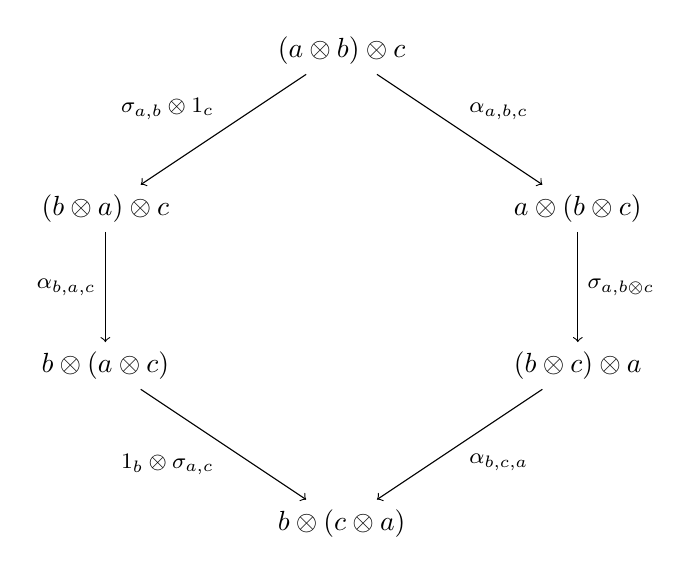
\begin{tikzpicture}
                \node (1) at (0, 0) {$(a\otimes b)\otimes c$};
                \node (2) at (-3, -2) {$(b\otimes a)\otimes c$};
                \node (3) at (3, -2) {$a\otimes(b\otimes c)$};
                \node (4) at (-3, -4) {$b\otimes (a\otimes c)$};
                \node (5) at (3, -4) {$(b\otimes c)\otimes a$};
                \node (6) at (0, -6) {$b\otimes(c\otimes a)$};
                \draw[->] (1) -- node[above left]{\footnotesize$\sigma_{a, b}\otimes\mathbbm{1}_c$} (2);
                \draw[->] (1) -- node[above right]{\footnotesize$\alpha_{a, b, c}$} (3);
                \draw[->] (2) -- node[left]{\footnotesize$\alpha_{b, a, c}$} (4);
                \draw[->] (3) -- node[right]{\footnotesize$\sigma_{a, b\otimes c}$} (5);
                \draw[->] (4) -- node[below left]{\footnotesize$\mathbbm{1}_b\otimes\sigma_{a, c}$} (6);
                \draw[->] (5) -- node[below right]{\footnotesize$\alpha_{b, c, a}$} (6);
            \end{tikzpicture}
            \caption{Hexagon diagram 1.}
            \label{fig:hexagon_diagrams1}
        \end{figure}
        \begin{figure}[ht!]
            \centering
            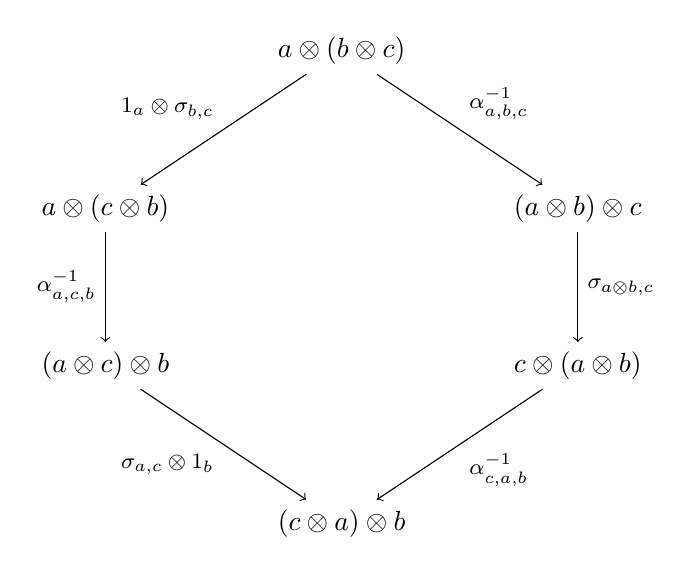
\begin{tikzpicture}
                \node (1) at (0, 0) {$a\otimes(b\otimes c)$};
                \node (2) at (-3, -2) {$a\otimes(c\otimes b)$};
                \node (3) at (3, -2) {$(a\otimes b)\otimes c$};
                \node (4) at (-3, -4) {$(a\otimes c)\otimes b$};
                \node (5) at (3, -4) {$c\otimes(a\otimes b)$};
                \node (6) at (0, -6) {$(c\otimes a)\otimes b$};
                \draw[->] (1) -- node[above left]{\footnotesize$\mathbbm{1}_a\otimes\sigma_{b, c}$} (2);
                \draw[->] (1) -- node[above right]{\footnotesize$\alpha^{-1}_{a, b, c}$} (3);
                \draw[->] (2) -- node[left]{\footnotesize$\alpha^{-1}_{a, c, b}$} (4);
                \draw[->] (3) -- node[right]{\footnotesize$\sigma_{a\otimes b, c}$} (5);
                \draw[->] (4) -- node[below left]{\footnotesize$\sigma_{a, c}\otimes\mathbbm{1}_b$} (6);
                \draw[->] (5) -- node[below right]{\footnotesize$\alpha^{-1}_{c, a, b}$} (6);
            \end{tikzpicture}
            \caption{Hexagon diagram 2.}
            \label{fig:hexagon_diagrams2}
        \end{figure}
    }
    \begin{property}[Yang-Baxter equation]\index{Yang-Baxter}
        The components $\sigma_{a,a}$ of a braiding satisfy the \textit{Yang-Baxter} equation. More generally, the braiding $\sigma$ satisfies the following equation for all objects $a,b,c\in\ob{C}$:
        \begin{gather}
            (\sigma_{b,c}\otimes\mathbbm{1}_a)\circ(\mathbbm{1}_b\otimes\sigma_{a,c})\circ(\sigma_{a,b}\otimes\mathbbm{1}_c) = (\mathbbm{1}_c\otimes\sigma_{a,b})\circ(\sigma_{a,c}\otimes\mathbbm{1}_b)\circ(\mathbbm{1}_a\otimes\sigma_{b,c}).
        \end{gather}
    \end{property}
    \remark{When drawing the above equality using string diagrams we see that the Yang-Baxter equation corresponds to the invariance of string diagrams under a \textit{Reidemeister III move}.\index{Reidemeister move}}

    \newdef{Symmetric monoidal category}{\label{cat:symmetric}
        A braided monoidal category where the braiding $\sigma$ satisfies
        \begin{gather}
            \sigma_{x,y}\circ\sigma_{y,x} = \mathbbm{1}_{x\otimes y}.
        \end{gather}
    }

    In chapter \ref{chapter:hda} the theory of monoidal categories is continued.

\subsection{Monoidal functors}

    \newdef{Monoidal functor}{\index{monoidal!functor}\index{coherence!maps}
        Let $(\mathbf{C},\otimes,\mathbf{1}_C), (\mathbf{D},\circledast,\mathbf{1}_D)$ be two monoidal categories. A functor $\func{F}{C}{D}$ is said to be monoidal if there exists:
        \begin{enumerate}
            \item A natural isomorphism $\psi_{a, b}: Fa\circledast Fb\Rightarrow F(a\otimes b)$ such that diagram \ref{fig:monoidal_functor1} commutes.

                \begin{figure}[ht!]
                    \centering
                    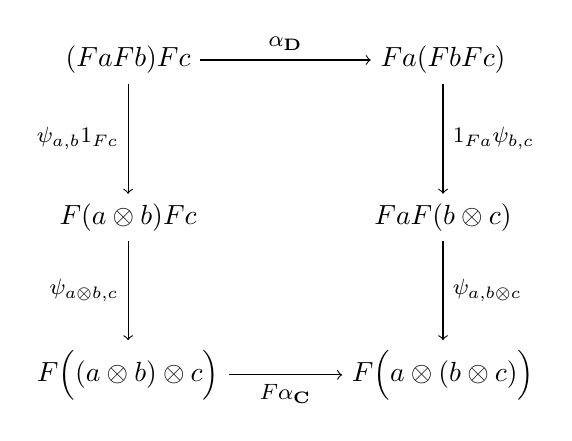
\begin{tikzpicture}
                        \node (1) at (0, 0) {$(Fa\circledast Fb)\circledast Fc$};
                        \node (2) at (4, 0) {$Fa\circledast(Fb\circledast Fc)$};
                        \node (3) at (0, -2) {$F(a\otimes b)\circledast Fc$};
                        \node (4) at (4, -2) {$Fa\circledast F(b\otimes c)$};
                        \node (5) at (0, -4) {$F\Big((a\otimes b)\otimes c\Big)$};
                        \node (6) at (4, -4) {$F\Big(a\otimes (b\otimes c)\Big)$};
                        \draw[->] (1) -- node[above]{\footnotesize$\alpha_{\mathbf{D}}$} (2);
                        \draw[->] (5) -- node[below]{\footnotesize$F\alpha_{\mathbf{C}}$} (6);
                        \draw[->] (1) -- node[left]{\footnotesize$\psi_{a, b}\circledast\mathbbm{1}_{Fc}$} (3);
                        \draw[->] (3) -- node[left]{\footnotesize$\psi_{a\otimes b, c}$} (5);
                        \draw[->] (2) -- node[right]{\footnotesize$\mathbbm{1}_{Fa}\circledast\psi_{b, c}$} (4);
                        \draw[->] (4) -- node[right]{\footnotesize$\psi_{a, b\otimes c}$} (6);
                    \end{tikzpicture}
                    \caption{Monoidal functor.}
                    \label{fig:monoidal_functor1}
                \end{figure}
            \item An isomorphism $\phi: \mathbf{1}_D\rightarrow F\mathbf{1}_C$ that makes the two diagrams in figure \ref{fig:unitality} commute.

            \begin{figure}[ht!]
                \centering
                \begin{subfigure}[b]{0.49\textwidth}
                    \centering
                    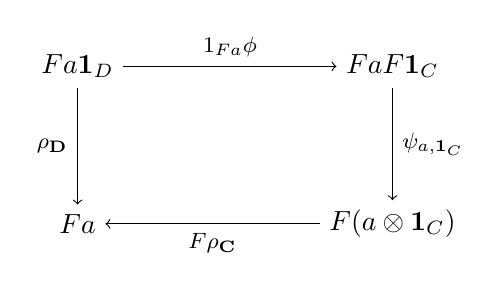
\begin{tikzpicture}
                        \node (1) at (0, 0) {$Fa\circledast\mathbf{1}_D$};
                        \node (2) at (4, 0) {$Fa\circledast F\mathbf{1}_C$};
                        \node (3) at (0, -2) {$Fa$};
                        \node (4) at (4, -2) {$F(a\otimes\mathbf{1}_C)$};
                        \draw[->] (1) -- node[above]{\footnotesize$\mathbbm{1}_{Fa}\circledast\phi$} (2);
                        \draw[<-] (3) -- node[below]{\footnotesize$F\rho_{\mathbf{C}}$} (4);
                        \draw[->] (1) -- node[left]{\footnotesize$\rho_{\mathbf{D}}$} (3);
                        \draw[->] (2) -- node[right]{\footnotesize$\psi_{a, \mathbf{1}_C}$} (4);
                    \end{tikzpicture}
                \end{subfigure}
                \begin{subfigure}[b]{0.49\textwidth}
                    \centering
                    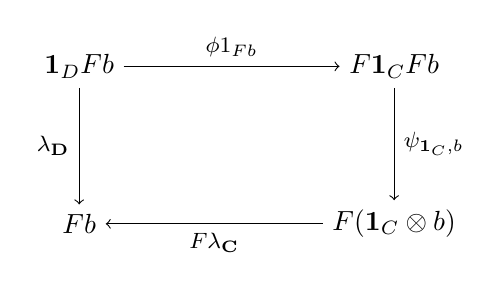
\begin{tikzpicture}
                        \node (1) at (0, 0) {$\mathbf{1}_D\circledast Fb$};
                        \node (2) at (4, 0) {$F\mathbf{1}_C\circledast Fb$};
                        \node (3) at (0, -2) {$Fb$};
                        \node (4) at (4, -2) {$F(\mathbf{1}_C\otimes b)$};
                        \draw[->] (1) -- node[above]{\footnotesize$\phi\circledast\mathbbm{1}_{Fb}$} (2);
                        \draw[<-] (3) -- node[below]{\footnotesize$F\lambda_{\mathbf{C}}$} (4);
                        \draw[->] (1) -- node[left]{\footnotesize$\lambda_{\mathbf{D}}$} (3);
                        \draw[->] (2) -- node[right]{\footnotesize$\psi_{\mathbf{1}_C, b}$} (4);
                    \end{tikzpicture}
                \end{subfigure}
                \caption{Unitality diagrams.}
                \label{fig:unitality}
            \end{figure}
        \end{enumerate}
    }
    \remark{The morphisms $\psi_{a,b}$ and $\phi$ are also called \textbf{coherence maps} or \textbf{structure morphisms}.}

    \begin{property}[Canonical unit]
        For every monoidal functor $F$ there exists in fact a canonical isomorphism $\phi:\mathbf{1}_D\rightarrow F\mathbf{1}_C$ defined by the commutative diagram \ref{fig:canonical_monoidal_isom}.
        \begin{figure}[ht!]
            \centering
            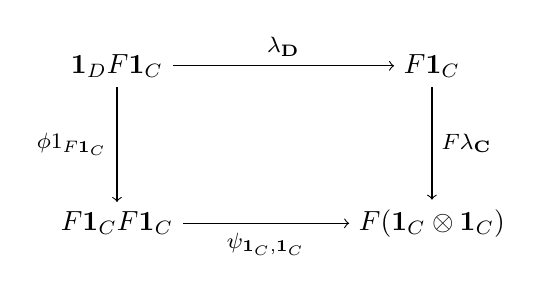
\begin{tikzpicture}
                \node (1) at (0, 0) {$\mathbf{1}_D\circledast F\mathbf{1}_C$};
                \node (2) at (4, 0) {$F\mathbf{1}_C$};
                \node (3) at (0, -2) {$F\mathbf{1}_C\circledast F\mathbf{1}_C$};
                \node (4) at (4, -2) {$F(\mathbf{1}_C\otimes\mathbf{1}_C)$};
                \draw[->] (1) -- node[above]{\footnotesize$\lambda_{\mathbf{D}}$} (2);
                \draw[->] (3) -- node[below]{\footnotesize$\psi_{\mathbf{1}_C, \mathbf{1}_C}$} (4);
                \draw[->] (1) -- node[left]{\footnotesize$\phi\circledast\mathbbm{1}_{F\mathbf{1}_C}$} (3);
                \draw[->] (2) -- node[right]{\footnotesize$F\lambda_{\mathbf{C}}$} (4);
            \end{tikzpicture}
            \caption{Canonical unit isomorphism.}
            \label{fig:canonical_monoidal_isom}
        \end{figure}
    \end{property}

    \newdef{Lax monoidal functor}{\index{lax!monoidal functor}
        A monoidal functor for which the coherence maps are merely morphisms and not isomorphisms.
    }

    \newdef{Monoidal natural transformation}{
        A natural transformation $\eta$ between (lax) monoidal functors $(F,\psi,\phi_F)$ and $(G,\widetilde{\psi},\phi_G)$ that makes the diagrams in figure \ref{fig:monoidal_natural_transformation} commute.
        \begin{figure}[ht!]
            \centering
            \begin{subfigure}[b]{0.49\textwidth}
                \centering
                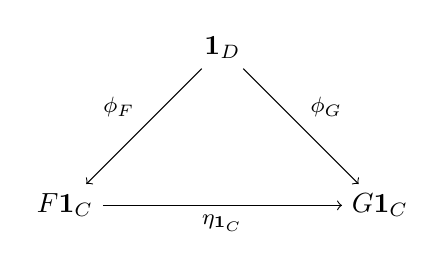
\begin{tikzpicture}
                    \node (1) at (0, 0) {$\mathbf{1}_D$};
                    \node (2) at (-2, -2) {$F\mathbf{1}_C$};
                    \node (3) at (2, -2) {$G\mathbf{1}_C$};
                    \draw[->] (1) -- node[above left]{\footnotesize$\phi_F$} (2);
                    \draw[->] (1) -- node[above right]{\footnotesize$\phi_G$} (3);
                    \draw[->] (2) -- node[below]{\footnotesize$\eta_{\mathbf{1}_C}$} (3);
                \end{tikzpicture}
            \end{subfigure}
            \begin{subfigure}[b]{0.49\textwidth}
                \centering
                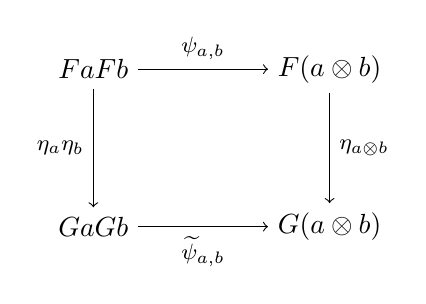
\begin{tikzpicture}
                    \node (1) at (0, 0) {$Fa\circledast Fb$};
                    \node (2) at (3, 0) {$F(a\otimes b)$};
                    \node (3) at (0, -2) {$Ga\circledast Gb$};
                    \node (4) at (3, -2) {$G(a\otimes b)$};
                    \draw[->] (1) -- node[above]{\footnotesize$\psi_{a, b}$} (2);
                    \draw[->] (3) -- node[below]{\footnotesize$\widetilde{\psi}_{a, b}$} (4);
                    \draw[->] (1) -- node[left]{\footnotesize$\eta_a\circledast\eta_b$} (3);
                    \draw[->] (2) -- node[right]{\footnotesize$\eta_{a\otimes b}$} (4);
                \end{tikzpicture}
            \end{subfigure}
            \caption{Monoidal natural transformation.}
            \label{fig:monoidal_natural_transformation}
        \end{figure}
    }

    \newdef{Monoidal equivalence}{\index{monoidal!equivalence}
        An equivalence of monoidal categories consisting of monoidal functors and monoidal natural isomorphisms.
    }
    \begin{theorem}[MacLane strictness theorem]\index{MacLane!strictness theorem}
        Every monoidal category is monoidally equivalent to a strict monoidal category.
    \end{theorem}

\section{Internal structures}\index{internal}

    \begin{property}[Eckmann-Hilton]\index{Eckmann-Hilton}\label{category:eckmann_hilton}
        A monoid internal to the category of monoids is the same as a commutative monoid. (See also property \ref{set:eckmann_hilton}.)
    \end{property}

    \newdef{Internal category}{\label{cat:internal_category}
        Let $\mathcal{E}$ be a category with pullbacks. A category $\mathbf{C}$ internal to $\mathcal{E}$ consists of the following data:
        \begin{enumerate}
            \item an object $C_0\in\ob{\mathcal{E}}$ of objects,
            \item an object $C_1\in\ob{\mathcal{E}}$ of morphisms,
            \item source and target morphisms $s, t\in\mathcal{E}(C_1, C_0)$,
            \item an ''identity-assigning'' morphism $e\in\mathcal{E}(C_0, C_1)$ such that \[s\circ e = \mathbbm{1}_{C_0}\qquad\qquad\qquad t\circ e = \mathbbm{1}_{C_0},\] and
            \item a composition morphism $c:C_1\times_{C_0}C_1\rightarrow C_1$ such that the following equations hold:
            \begin{align*}
                s\circ c = s\circ\pi_1\qquad\qquad&\qquad\qquad t\circ c = t\circ\pi_2\\
                \pi_1 = c\circ(e\times_{C_0}\mathbbm{1})\qquad\qquad&\qquad\qquad c\circ(\mathbbm{1}\times_{C_0}e)=\pi_2\\
                c\circ(c\times_{C_0}\mathbbm{1}) &= c\circ(\mathbbm{1}\times_{C_0}c)
            \end{align*}
            where $\pi_1,\pi_2$ are the canonical projections associated with the pullback $C_1\times_{C_0}C_1$ of $(s,t)$.
        \end{enumerate}

        Morphisms between these categories, suitably called \textbf{internal functors}, are given by a pair of morphisms (in $\mathcal{E}$) between internal objects and morphisms, that preserve composition and identities. Internal natural transformations are defined in a similar way.
    }
    \begin{notation}
        The \textit{(bi)category} of internal categories in $\mathcal{E}$ is denoted by $\mathbf{Cat}(\mathcal{E})$. It should be noted that for $\mathcal{E}=\mathbf{Set}$ we obtain $\mathbf{Cat}(\mathbf{Set})=\mathbf{Cat}$, i.e. the ordinary \textit{(bi)category} of small categories.
    \end{notation}
    \begin{adefinition}
        The above definition can be reformulated in a very elegant way: An internal category in $\mathcal{E}$ is a monad in the bicategory $\mathbf{Span}(\mathcal{E})$ of spans in $\mathcal{E}$.
    \end{adefinition}

    Functors between internal categories are not the only relevant morphisms. If we want to define (co)presheafs such as the hom-functor, we stumble upon a problem. In $\mathbf{Cat}$ we had, by definition, maps to the ambient (ordinary category theory has a set-theoretic foundation) category $\mathbf{Set}$. However, for internal categories there does not necessarily exist a morphism $\mathbf{D}\rightarrow\mathcal{E}$. To solve this problem we can consider a more general structure:
    \newdef{Internal diagram}{\index{diagram}
        A left module over a monad in $\mathbf{Span}(\mathcal{E})$. The dual notion is better known as an \textbf{internal presheaf}.
    }
    This is in fact a specific instance of an even more general concept (for more information on the definitions and applications see \cite{maclane, johnstone}):
    \newdef{Internal profunctor}{\index{pro!functor}
        A bimodule between monads in $\mathbf{Span}(\mathcal{E})$.
    }

    \begin{construct}[Internal Yoneda profunctor]
        Consider an internal functor $\func{F}{C}{D}$. This functor induces two internal profunctors $\profunc{F_*}{D}{C}$ and $\profunc{F^*}{C}{D}$. If we expand the definition using spans, we can define these profunctors as follows:

        \qquad For $F_*$ we define the object map as $(F_*)_0:C_0\times_{D_0} D_1:C_0\times D_0$. The action of $f\in D_1$ is given by postcomposition with $f$ in the second factor, while the action of $g\in C_1$ is given by precomposition with $Fg$ in the second factor (and changing to the domain of $g$ in the first factor).

        It can easily be shown that the profunctors induced by an identity functor $\text{id}_{\mathbf{C}}$ are isomorphic. In the case of $\mathcal{E}=\mathbf{Set}$ it can also be shown that this profunctor is exactly the hom-functor. Therefore we call this functor in general the (internal) Yoneda profunctor $Y(\mathbf{C})$.
    \end{construct}

\subsection{Closed categories}

    \newdef{Internal hom}{\index{internal!hom}\label{category:internal_hom}
        Let $(\mathbf{M},\otimes,\mathbf{1})$ be a monoidal category. In this setting we can generalize the \textit{currying} procedure, i.e. the identification of maps $x\times y\rightarrow z$ with maps $x\rightarrow(y\rightarrow z)$. The ''internal'' hom-functor is defined by the following natural isomorphism:
        \begin{gather}
            \hom(x\otimes y, z)\cong\hom(x, \underline{\hom}(y, z)).
        \end{gather}
        The existence of all internal homs is equivalent to the existence of a right adjoint to the tensor functor.
    }
    \begin{notation}
        The internal hom $\underline{\hom}(a, b)$ is also often denoted by $[a,b]$. From now on we will follow this convention (unless otherwise specified).
    \end{notation}
    \newdef{Closed monoidal category}{\index{closed!category}\index{Cartesian!closed}\label{cat:closed}
        A monoidal category $(\mathbf{C},\otimes,\mathbf{1})$ is said to be closed monoidal if it has all internal homs. If the monoidal structure is induced by a (Cartesian) product structure, the category is often called a \textbf{Cartesian closed category}.

        A category for which all slice categories are Cartesian closed is said to be locally Cartesian closed. If it contains a terminal object, it is automatically Cartesian closed itself.
    }

    \newdef{Exponential object}{\index{exponential!object}\label{category:exponential_object}
        In the case of Cartesian (monoidal) categories, i.e. categories where the monoidal structure is given by the (Cartesian) product, the internal hom $\underline{\text{Hom}}(a, b)$ is called the exponential object. This object is often denoted by $b^a$.
    }
    \begin{notation}
        In Cartesian closed categories a different, but frequently used, notation is $a\Rightarrow b$. However, we will not use this as it might confuse with the notation for \textit{2-morphisms}.
    \end{notation}

    \newdef{Cartesian closed functor}{\index{Cartesian!closed}\label{cat:cartesian_closed_functor}
        A functor between Cartesian closed categories that preserves products and exponential objects. (As such it is the natural notion of functor between Cartesian closed categories.)
    }
    \begin{property}[Frobenius reciprocity]\index{Forbenius!reciprocity}
        A functor $R$ between Cartesian closed categories that admits a left adjoint $L$ is Cartesian closed if and only if the natural transformation
        \begin{gather}
            L(b\times Ra)\rightarrow Lb\times a
        \end{gather}
        is in fact a natural isomorphism.
    \end{property}

    \begin{property}[Global elements]\label{cat:internal_hom_property}
        The following isomorphism is natural in both $a,b\in\ob{M}$:
        \begin{gather}
            \mathbf{M}(\mathbf{1}, [a,b])\cong\mathbf{M}(a, b).
        \end{gather}
        It is this relation that gives the best explanation for the term ''internal hom''. We also immediately obtain the following natural isomorphism:
        \begin{gather}
            \mathbf{M}(a, [\mathbf{1},b])\cong\mathbf{M}(a, b).
        \end{gather}
        Because the Yoneda embedding is fully faithful this implies that $[\mathbf{1},b]\cong b$. Although the ''global'' elements $\mathbf{M}(\mathbf{1}, b)$ do not fully specify an object $b$, this does hold internally.
    \end{property}

    \begin{property}[Symmetry]
        Let $\mathbf{M}$ be a closed monoidal category. The definition of an internal hom can also be internalized, i.e. there exists a natural isomorphism of the form
        \begin{gather}
            [a\otimes b,c]\cong[a,[b,c]].
        \end{gather}
        Furthermore, if $\mathbf{M}$ is also symmetric \ref{cat:symmetric}, there exists an internal isomorphism of the form
        \begin{gather}
            \label{cat:internal_symmetry}
            [a,[b,c]]\cong[b,[a,c]].
        \end{gather}
    \end{property}

    \newdef{Strong adjunction}{\index{adjunction!strong}
        Consider a monoidal category $\mathbf{M}$ together with two endofunctors $\func{L,R}{M}{M}$. These functors are said to form a strong adjunction if there exists a natural isomorphism
        \begin{gather}
            [La,b]\cong[a,Rb].
        \end{gather}
        Property \ref{cat:internal_hom_property} above implies that every strong adjunction is in particular an adjunction in the sense of section \ref{section:adjunction}.
    }

\section{Enriched category theory}\label{section:enriched_category_theory}

    \newdef{Cosmos}{\index{cosmos}\label{cat:cosmos}
        A complete and cocomplete closed symmetric monoidal category.
    }

    \newdef{Enriched category}{\index{category!enriched}
            Let $(\mathcal{V}, \otimes, \mathbf{1})$ be a monoidal category. A $\mathcal{V}$-enriched category, also called a $\mathcal{V}$-category\footnote{Not to be confused with the notation for fibre categories \ref{cat:fibre_category}.}, consists of the following elements:
            \begin{enumerate}
                \item a collection of objects $\ob{C}$, and
                \item for every pair of objects $a,b\in\ob{C}$, an object $\mathbf{C}(a, b)\in\ob{\mathcal{V}}$ for which the following morphisms exist:
                \begin{itemize}
                    \item $\text{id}_a: \mathbf{1}\rightarrow\mathbf{C}(a, a)$ giving the (enriched) identity morphism, and
                    \item $\circ_{abc}:\mathbf{C}(b, c)\otimes\mathbf{C}(a, b)\rightarrow\mathbf{C}(a, c)$ replacing the usual composition.
                \end{itemize}
            \end{enumerate}
            The associativity and unity properties are given by commutative diagrams for the $\text{id}$ and $\circ$ morphisms together with the associators and unitors in $\mathcal{V}$.
    }
    \newdef{Underlying category}{
        Given a $\mathcal{V}$-enriched category $\mathbf{C}$ we define the underlying category $\mathbf{C}_0$ as follows:
        \begin{itemize}
            \item $\text{ob}(\mathbf{C}_0):=\ob{C}$, and
            \item $\mathbf{C}_0(x, y):=\mathcal{V}(\mathbf{1}, \mathbf{C}(x, y))$
        \end{itemize}
        where $\mathbf{1}$ is the monoidal unit in $\mathcal{V}$. This construction can be obtained as the functor $\mathcal{V}\mathbf{Cat}(\mathcal{I}, -)$ where $\mathcal{I}$ is the one-object $\mathcal{V}$-category with $\mathcal{I}(\ast,\ast)\equiv\mathbf{1}$.
    }
    \begin{property}[$\mathcal{V}$ as a $\mathcal{V}$-category]
        Consider a closed monoidal category $\mathcal{V}$. This category can be given the structure $\widetilde{\mathcal{V}}$ of a $\mathcal{V}$-category by taking the hom-objects to be the internal homs, i.e. $\widetilde{\mathcal{V}}(x, y) := [x, y]$ for all $x,y\in\mathcal{V}$. Property $\ref{cat:internal_hom_property}$ then implies that there exists an isomorphism between the underlying category $\widetilde{\mathcal{V}}_0$ and the original category $\mathcal{V}$.
    \end{property}

    Given two $\mathcal{V}$-enriched categories we can define suitable functors between them:
    \newdef{Enriched functor}{\index{functor}
        A $\mathcal{V}$-enriched functor $\func{F}{C}{D}$ consists of the following data:
        \begin{enumerate}
            \item a function $F_0:\ob{C}\rightarrow\ob{D}$ (as for ordinary functors), and
            \item for every two objects $a,b\in\ob{C}$, a morphism $F_{a,b}:\mathbf{C}(a, b)\rightarrow\mathbf{D}(Fa, Fb)$ in $\mathcal{V}$.
        \end{enumerate}
        These have to satisfy the ''usual'' composition and unit conditions.

        By extending the property \ref{cat:natural_end} using enriched ends, we obtain a definition of enriched natural transformations and threfore also a definition of enriched functor categories.:
        \begin{gather}
            \funccat{C}{D}(F, G) := \int_{c\in\mathbf{C}}\mathbf{D}(Fc, Gc).
        \end{gather}
    }
    Given two $\mathcal{V}$-enriched functors $\func{F,G}{C}{D}$ we can also try to define $\mathcal{V}$-natural transformations by extending the usual definition of natural transformations \ref{cat:natural}:
    \newdef{Enriched natural transformation}{\index{natural!transformation}
         An ordinary natural transformation consists of a $\ob{C}$-indexed family of morphism $\eta_c:Fc\rightarrow Gc$. This can also be interpreted as a $\ob{C}$-indexed family of morphisms $\eta_c:1\rightarrow\mathbf{D}(Fc, Gc)$ from the initial one-object set. Therefore we define a $\mathcal{V}$-natural transformation as a $\ob{C}$-indexed family of morphisms $\eta_c:\mathbf{1}\rightarrow\mathbf{D}(Fc, Gc)$ from the monoidal unit. The usual naturality square is no replaced by the naturality hexagon \ref{fig:v_naturality}.

        The question then becomes how we can relate these to the morphism in the enriched functor category $\funccat{C}{D}$. The above end comes equipped with a counit $\varepsilon_c:\funccat{C}{D}(F, G)\rightarrow\mathbf{D}(Fc, Gc)$. Precomposing this counit with a morphism in the underlying category, i.e. an element of $\mathcal{V}(\mathbf{1}, \funccat{C}{D}(F, G))$, gives us exactly a $\mathcal{V}$-natural transformation. We conclude that the underlying category of $\funccat{C}{D}$ is the ordinary category of $\mathcal{V}$-functors and $\mathcal{V}$-natural transformations.

         \begin{figure}
            \centering
            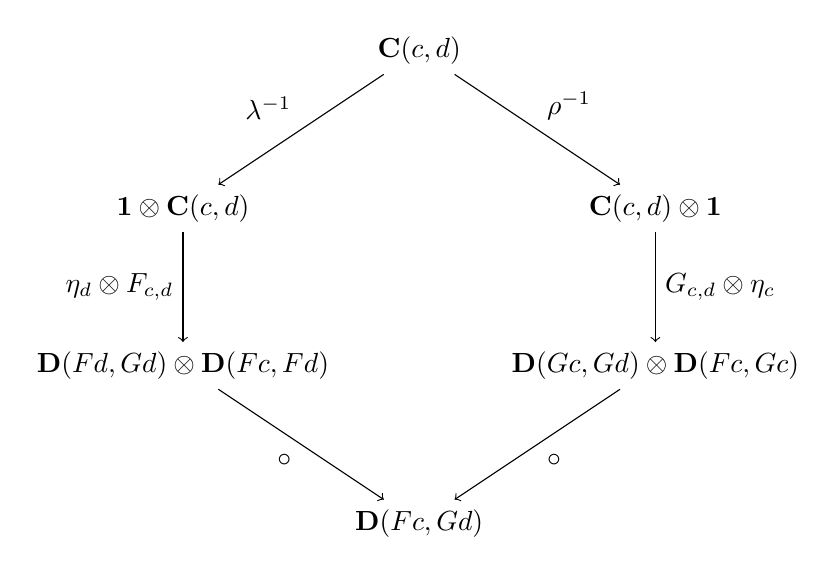
\begin{tikzpicture}
                \node (C) at (0, 0) {$\mathbf{C}(c, d)$};
                \node (IC) at (-3, -2) {$\mathbf{1}\otimes\mathbf{C}(c, d)$};
                \node (CI) at (3, -2) {$\mathbf{C}(c, d)\otimes\mathbf{1}$};
                \node (DF) at (-3, -4) {$\mathbf{D}(Fd, Gd)\otimes\mathbf{D}(Fc, Fd)$};
                \node (DG) at (3, -4) {$\mathbf{D}(Gc, Gd)\otimes\mathbf{D}(Fc, Gc)$};
                \node (D) at (0, -6) {$\mathbf{D}(Fc, Gd)$};
                \draw[->] (C) -- node[above left]{$\lambda^{-1}$} (IC);
                \draw[->] (C) -- node[above right]{$\rho^{-1}$} (CI);
                \draw[->] (IC) -- node[left]{$\eta_d\otimes F_{c,d}$} (DF);
                \draw[->] (CI) -- node[right]{$G_{c,d}\otimes\eta_c$} (DG);
                \draw[->] (DF) -- node[below left]{$\circ$} (D);
                \draw[->] (DG) -- node[below right]{$\circ$} (D);
            \end{tikzpicture}
            \caption{$\mathcal{V}$-naturality diagram.}
            \label{fig:v_naturality}
         \end{figure}
    }

\subsection{Enriched constructions}

    \newdef{Functor tensor product}{\index{tensor!product}\label{cat:functor_tensor_product}
        Consider a covariant functor $\func{G}{C}{M}$ and a contravariant functor $\cfunc{F}{C}{M}$ into a monoidal category $\mathbf{M}$. ($\mathbf{C}$ does not have to be enriched over $\mathbf{M}$.) The tensor product of $F$ and $G$ is defined as the following coend:
        \begin{gather}
            F\otimes_{\mathbf{C}} G := \int^{c\in\mathbf{C}}Fc\otimes Gc.
        \end{gather}
    }
    It should be noted that the above tensor product does not produce a new functor, instead it only gives an object in $\mathbf{M}$. A different type of tensor product, one that does give a functor, exists in the enriched setting (note that there is no relation between these two definitions):
    \newdef{Day convolution}{\index{Day convolution}
        Consider a monoidally cocomplete category\footnote{A cocomplete monoidal category for which the tensor product bifunctor is cocontinuous in each argument.} $\mathbf{M}$ together with a $\mathbf{M}$-enriched category $\mathbf{C}$. Given two $\mathbf{M}$-enriched functors $\func{F,G}{C}{M}$ we define their tensor product (if it exists) as the following coend:
        \begin{gather}
            F\otimes_{\text{Day}} G := \iint^{x,y\in\mathbf{C}}\mathbf{C}(x\otimes y, -)\otimes Fx\otimes Gy.
        \end{gather}
    }
    \begin{property}[Monoidal structure]
        In the case that $\mathbf{M}$ is a closed symmetric monoidal category the Day convolution is associative and hence defines a monoidal structure on the functor category $[\mathbf{C},\mathbf{M}]$. The tensor unit is given by the functor (co)represented by the tensor unit in $\mathbf{C}$.
    \end{property}

    \newdef{Copower}{\index{co-!power}\index{power} % Both terms are indexed since copowers are rather important on their own.
        Consider a $\mathcal{V}$-enriched category $\mathbf{C}$. We define the copower (or tensor) functor $\func{\cdot}{\mathcal{V}\times C}{C}$ by the following natural isomorphism:
        \begin{gather}
            \mathbf{C}(v\cdot c, c')\cong[v,\mathbf{C}(c, c')]
        \end{gather}
        where the brackets $[-,-]$ on the right-hand side denote the internal Hom in $\mathcal{V}$. Dually, we define the power (or cotensor) functor $\func{[-,-]}{\mathcal{V}\times C}{C}$ by the following natural isomorphism:
        \begin{gather}
            \mathbf{C}(c, [v,c'])\cong[v,\mathbf{C}(c, c')]
        \end{gather}
        where the brackets $[-,-]$ on the right-hand side again denote the internal Hom in $\mathcal{V}$. If an enriched category admits all (co)powers, it is said to be \textbf{(co)powered} (over its enriching category).
    }
    \remark{Equation \ref{cat:internal_symmetry} says that every (closed) symmetric monoidal category $\mathbf{M}$ is powered over itself, the power object just being the internal hom. The same holds for the copower, which is just the usual tensor product functor.}

    \begin{example}[Disjoint unions]
        Every (co)complete (locally) small category $\mathbf{C}$ admits the structure of a $\mathbf{Set}$-(co)powered category:
        \begin{gather}
            c^S := \prod_{s\in S}c\\
            S\cdot c := \bigsqcup_{s\in S}c.
        \end{gather}
    \end{example}

    The definition and properties of internal hom-functors and (co)powers can be formalized as follows:
    \newdef{Two-variable adjunction}{\index{adjunction}\label{cat:two_variable_adjunction}
        Consider three categories $\mathbf{C, D}$ and $\mathbf{E}$. A two-variable adjunction $\mathbf{C}\times\mathbf{D}\rightarrow\mathbf{E}$ consists of three bifunctors:
        \begin{enumerate}
            \item $\func{-\otimes-}{C\times D}{E}$,
            \item $\text{hom}_L:\mathbf{C}^{op}\times\mathbf{E}\rightarrow\mathbf{D}$, and
            \item $\text{hom}_R:\mathbf{D}^{op}\times\mathbf{E}\rightarrow\mathbf{C}$
        \end{enumerate}
        admitting the following natural isomorphisms:
        \begin{gather}
            \mathbf{E}(c\otimes d, e)\cong\mathbf{C}(c, \text{hom}_R(d, e))\cong\mathbf{D}(d, \text{hom}_L(c, e)).
        \end{gather}
        It should be noted that fixing any of the variables gives rise to ordinary adjunctions in the sense of section \ref{section:adjunction}.
    }
    \begin{property}[Powers and copowers]
        A category $\mathbf{C}$ enriched over a monoidal category $\mathcal{V}$ is powered and copowered over $\mathcal{V}$ exactly if the hom-functor $\mathbf{C}^{op}\times\mathbf{C}\rightarrow\mathcal{V}$ is the right adjoint in an enriched two-variable adjunction. The power and copower functors are then given by the other two adjoints.
    \end{property}

    The following definition constructs Kan extensions in the enriched setting (these can be shown to reduce to \ref{cat:kan_extension} when enriching over $\mathbf{Set}$):
    \newadef{Kan extension}{\index{Kan!extension}\label{cat:enriched_kan_extension}
        Let $\mathbf{C}, \mathbf{D}$ and $\mathbf{E}$ be categories enriched over a monoidal category $\mathcal{V}$. If we assume that $\mathbf{D}$ is copowered over $\mathcal{V}$, then we can define the left Kan extension of $\func{F}{C}{D}$ along $\func{G}{C}{E}$ as a coend:
        \begin{gather}
            \text{Lan}_GF := \int^{c\in\mathbf{C}}\mathbf{E}(Gc, -)\otimes Fc.
        \end{gather}
        If we assume that $\mathbf{D}$ is powered over $\mathcal{V}$, then we can define the right Kan extension as an end:
        \begin{gather}
            \text{Ran}_GF := \int_{c\in\mathbf{C}}[\mathbf{E}(-, Gc), Fc].
        \end{gather}
    }
    \remark{By choosing $\mathcal{V}=\mathbf{Set}, \mathbf{E}=\mathbf{C}$ and $G=\text{id}_{\mathbf{C}}$ in the previous definition we exactly obtain the ninja Yoneda lemma \ref{cat:ninja_yoneda}.}
    \begin{property}
        Kan extensions computed using (co)ends as above are pointwise in the sense of definition \ref{cat:pointwise_kan_extension}.
    \end{property}

    \newadef{Functor tensor product}{\index{tensor!product}
        Let $\mathbf{D}$ be a category enriched over a monoidal category $\mathcal{V}$. Consider a covariant functor $\func{G}{C}{D}$ and a contravariant functor $\cfunc{F}{C}{\mathcal{V}}$. The tensor product \ref{cat:functor_tensor_product} can be generalized whenever $\mathbf{D}$ is copowered over $\mathcal{V}$:
        \begin{gather}
            \label{cat:copower_product}
            F\otimes_{\mathbf{C}} G := \int^{c\in\mathbf{C}}Fc\cdot Gc.
        \end{gather}
    }

\subsection{Weighted (co)limits}\index{limit!weighted}

    We now come back to the definition of ordinary limits and, in particular, its defining universal property \ref{cat:limit_uproperty}. In this construction the constant functor $\Delta_c$ was one of the main ingredients. This functor can be factorized as $\mathbf{I}\rightarrow1\rightarrow\mathbf{C}$ where $1$ denotes the terminal category. On the level of morphisms this factorization takes the form $\mathbf{I}(i, j)\rightarrow\ast\rightarrow\mathbf{C}(c, c)$ where $\ast$ denotes the terminal one-element set. However, whenever the enriching context is not $\mathbf{Set}$, we do not necessarily have access to a terminal object.

    First we will redefine limits as representing objects. To this end let us consider a general diagram $\func{D}{I}{C}$. By postcomposition with the Yoneda embedding we obtain the presheaf-valued diagram $\mathbf{C}(-, D-):\mathbf{I}\rightarrow[\mathbf{C}^{op}, \mathbf{Set}]$. Since presheaf categories are complete (example \ref{cat:complete_presheaf_category}), we can always find the limit of this diagram: \[\mathbf{Set}(s, \lim\mathbf{C}(c, D-))\cong\funccat{I}{Set}(\Delta_s, \mathbf{C}(c, D-)).\] If we restrict to the terminal set $s=\ast$, we obtain \[\lim\mathbf{C}(c, D-)\cong\funccat{I}{Set}(\Delta_\ast, \mathbf{C}(c, D-)).\] If this presheaf is representable, we can use the continuity of the covariant hom-functor, together with the fact that the Yoneda embedding is fully faithful, to show that the representing object is (isomorphic to) $\lim D$, i.e.
    \begin{gather}
        \funccat{I}{Set}(\Delta_\ast, \mathbf{C}(c, D-))\cong\mathbf{C}(c, \lim D).
    \end{gather}

    ?? CLEAN THIS UP (note that continuity and pointwise definition was already mentioned for ordinary limits) ??

    \newdef{Weighted limit}{\index{limit!conical}\label{cat:weighted_limit}
        We can now generalize this definition by replacing the constant functor $\Delta_\ast$ by any functor $\func{W}{I}{Set}$. A representing object is then called the $W$-weighted limit of $D$. This object is often denoted by $\wlim{W}D$ or $\{W,D\}$. To distinguish weighted limits from ordinary ones, we sometimes call the latter \textbf{conical limits}.
    }

    \begin{remark}
        A motivation for this construction is the following: As was already pointed out in remark \ref{cat:global_elements_remark}, the mere knowledge of global elements $1\rightarrow x$ is often not enough to characterize an object $x$. In general we should look at a collection of generalized elements. When applying this ideology to the case of cones, we see that replacing the functor $\Delta_\ast$ by a more general functor is the same as replacing the global elements $\ast\rightarrow Di$ by generalized elements $Wi\rightarrow Di$.
    \end{remark}

    The generalization to the enriched setting is now evident. There is no reference to the terminal object left, so we can replace $\mathbf{Set}$ by any enriching category. We will often use (co)end formulas for (weighted) limits, especially in the enriched setting:
    \newformula{Enriched weighted limits}{\label{cat:weighted_limits}
        By expressing the natural transformations as an end (see equation \ref{cat:natural_end}) and by using the canonical powering in $\mathbf{Set}$, we can express ordinary weighted limits as follows:
        \begin{gather}
            \wlim{W}D\cong\int_{i\in\mathbf{I}}[Wi,Di].
        \end{gather}
        The generalization to other enriching categories is now straightforward: Consider a diagram $\func{D}{I}{\mathcal{V}}$ and a weight functor $\func{W}{I}{C}$ where $\mathbf{C}$ is $\mathcal{V}$-enriched. If $\mathbf{C}$ is powered over $\mathcal{V}$, we define the $W$-weighted limit of $D$ by the same formula as above:
        \begin{gather}
            \wlim{W}D:=\int_{i\in I}[Wi,Di].
        \end{gather}
        In a similar way we can define weighted colimits in copowered $\mathcal{V}$-categories as coends:
        \begin{gather}
            \colim^WD:=\int^{i\in I}Wi\cdot Di.
        \end{gather}
        Here the weight functor $W$ is required to be contravariant since colimits (and cocones in general) are natural transformations between contravariant functors.
    }
    \begin{property}[Weighted limits are Hom-objects]
        If we take $\mathbf{C}=\mathcal{V}$, the powering functor becomes the internal Hom and therefore we obtain that weighted limits are given by (enriched) natural transformations (as was the case for ordinary conical limits).
    \end{property}

    In the following example we compute the weighted colimit with respect to the Yoneda embedding:
    \begin{example}[Hom-functor]
        Consider a diagram $\func{D}{I}{C}$. If we use the Yoneda embedding $\mathcal{Y}i = \mathbf{I}(-, i)$ as the weight functor, we obtain the following property by virtue of the Yoneda lemma:
        \begin{gather}
            \label{cat:weighted_hom_colimit}
            \colim^{\mathcal{Y}i}D\cong Di.
        \end{gather}
        A similar statement for weighted limits can be obtained with the covariant Yoneda embedding.
    \end{example}
    \newadef{Weighted (co)limits}{
        The above property can be used to axiomatize small weighted (co)limits in bicomplete categories:
        \begin{enumerate}
            \item \textbf{Yoneda}: For every object $i\in\ob{I}$ we obtain isomorphisms
            \begin{gather}
                \text{lim}^{\mathbf{I}(i, -)}D\cong Di\qquad\text{and}\qquad\text{colim}^{\mathbf{I}(-, i)}D\cong Di.
            \end{gather}
            \item \textbf{Cocontinuity}: The weighted (co)limit functors are cocontinuous in the weights.
        \end{enumerate}
    }

    We can also express Kan extensions as weighted limits:
    \begin{property}[Kan extensions]\index{Kan!extension}
        Consider functors $\func{F}{C}{D}$ and $\func{G}{C}{E}$. If for every $e\in\ob{E}$ the weighted limit $\wlim{\mathbf{E}(e, G-)}F$ exists, then these limits can be combined into a functor which can be shown to be the right Kan extension $\text{Ran}_GF$. The left Kan extension can be obtained through a weighted colimit.
    \end{property}

\section{Abelian categories}\label{section:abelian_categories}

    \newdef{Pre-additive category}{
        A (locally small) category enriched over $\mathbf{Ab}$, i.e. every hom-set is an Abelian group and composition is bilinear.
    }

    \begin{property}\index{zero!object}
        Let $\mathbf{A}$ be a pre-additive category. The following statements are equivalent for an object $a\in\ob{A}$:
        \begin{itemize}
            \item $a$ is initial,
            \item $a$ is final, or
            \item $\mathbbm{1}_a = 0$.
        \end{itemize}
        It follows that every initial/terminal object in a pre-additive category is automatically a zero object \ref{cat:zero_object}.
    \end{property}
    \begin{property}[Biproducts]\index{biproduct}\index{direct!sum}
        In a pre-additive category the following isomorphism holds for all finitely indexed sets $\{x_i\}_{i\in I}$:
        \begin{gather}
            \prod_{i\in I}x_i \cong \bigsqcup_{i\in I}x_i.
        \end{gather}
        Finite (co)products in pre-additive categories are often called \textbf{direct sums}. In general, if a product and coproduct exist and are equal, one also speaks of a \textbf{biproduct}.
    \end{property}

    \newdef{Additive category}{\index{additive!category}
        A pre-additive category in which all finite products exist.
    }

    When working with additive categories, we generally assume that the associated functors are of a specific type:
    \newdef{Additive functor}{\index{additive!functor}\label{category:additive_functor}
        Let $\mathbf{A},\mathbf{A'}$ be additive categories. A functor $\func{F}{A}{A'}$ is said to be additive if it preserves finite biproducts:
        \begin{enumerate}
            \item It preserves zero objects: $F0_{\mathbf{A}} \cong 0_{\mathbf{A}'}$.
            \item There exists a natural isomorphism $F(x\oplus y)\cong Fx\oplus Fy$ for all $x,y\in\ob{A}$.
        \end{enumerate}
        We can generalize this notion to pre-additive categories. A functor between pre-additive categories is said to be additive if it acts as a group morphism on hom-spaces.
    }

    \newdef{Grothendieck group}{\index{Grothendieck!group}
        Let $\mathbf{A}$ be an additive category and consider its decategorification $\text{Decat}(\mathbf{A})$. This set carries the structure of an Abelian monoid and hence we can apply the Grothendieck construction \ref{group:grothendieck_completion} to obtain an Abelian group $K(\mathbf{A})$. This group is called the Grothendieck group of $\mathbf{A}$.
    }

    In a (pre-)additive category we can define the classical notions from (homological) algebra such as images and kernels:
    \newdef{Kernel}{\index{kernel}
        Let $f:x\rightarrow y$ be a morphism. A\footnote{Note the word ''\textit{a}''. The kernel of a morphism is only determined up to an isomorphism.} kernel is a morphism $k:z\rightarrow x$ such that:
        \begin{enumerate}
            \item $f\circ k = 0$.
            \item \textbf{Universal property}: For every morphism $k':z'\rightarrow x$ such that $f\circ k' = 0$ there exists a unique morphism $h:z'\rightarrow z$ such that $k\circ h = k'$.
        \end{enumerate}
        This implies that a kernel of $f$ is an equalizer of $f$ and $0$.
    }
    \begin{notation}[Kernel]
        If the kernel of $f:x\rightarrow y$ exists, then it is denoted by $\ker(f)$.
    \end{notation}

    \newdef{Cokernel}{
        Let $f:x\rightarrow y$ be a morphism. A cokernel is a morphism $p:y\rightarrow z$ such that:
        \begin{enumerate}
            \item $p\circ f = 0$.
            \item \textbf{Universal property}: For every morphism $p':y\rightarrow z'$ such that $p'\circ f = 0$ there exists a unique morphism $h:z\rightarrow z'$ such that $h\circ p = p'$.
        \end{enumerate}
        This implies that a cokernel of $f$ is a coequalizer of $f$ and 0.
    }
    \begin{notation}[Cokernel]
        If the cokernel of $f:x\rightarrow y$ exists, then it is denoted by $\text{coker}(f)$.
    \end{notation}
    \begin{remark}
        The name and notation of the kernel\footnote{Similarly for the cokernel.} (in the categorical sense) is explained by remarking that $\ker(f)$ represents the functor \[F:z\mapsto\ker\Big(\mathbf{C}(z, x)\rightarrow\mathbf{C}(z, y)\Big)\] where $\ker$ in the second line denotes the algebraic kernel \ref{group:kernel}.
    \end{remark}

    \newdef{Pseudo-Abelian category}{\label{category:pseudo_abelian}
        An additive category in which every projection (a morphism $p$ such that $p^2=p$) has a kernel.
    }
    \newdef{Pre-Abelian category}{
        An additive category in which every morphism has a kernel and cokernel.
    }
    \newdef{Abelian category}{\index{Abelian!category}
        A pre-Abelian category in which every mono is a kernel and every epi is a cokernel or, equivalently, if for every morphism $f$ there exists an isomorphism
        \begin{gather}
            \text{coker}(\ker(f))\cong\ker(\text{coker}(f)).
        \end{gather}
    }

    \begin{property}[Injectivity and surjectivity]
        In Abelian categories a morphism is monic if and only if it is injective, i.e. its kernel is 0. Analogously, a morphism is epic if and only if it is surjective, i.e. its cokernel is 0.
    \end{property}

    \newdef{$k$-linear category}{\index{category!linear}
        Let $\textbf{Vect}_k$ denote the category of vector spaces over the base field $k$. A $k$-linear category is a category enriched over $\textbf{Vect}_k$. (If the base field is clear, the subscript is often left implicit.)
    }

    \newdef{Exact functor}{\index{exact!functor}
        Let $\func{F}{A}{A'}$ be an additive functor between additive categories. We use the following definitions:
        \begin{itemize}
            \item $F$ is said to be left exact if it preserves kernels.
            \item $F$ is said to be right exact if it preserves cokernels.
            \item $F$ is said to be exact if it is both left and right exact.
        \end{itemize}
    }
    \begin{result}
        The previous definition implies the following properties (which can in fact be used as an alternative definition):
        \begin{itemize}
            \item If $F$ is left exact, it maps an exact sequence of the form \[0\longrightarrow a\longrightarrow b\longrightarrow c\]
            to an exact sequence of the form \[0\longrightarrow Fa\longrightarrow Fb\longrightarrow Fc.\]
            \item If $F$ is right exact, it maps an exact sequence of the form \[a\longrightarrow b\longrightarrow c\longrightarrow 0\]
            to an exact sequence of the form \[Fa\longrightarrow Fb\longrightarrow Fc\longrightarrow 0.\]
            \item If $F$ is exact, it maps short exact sequences to short exact sequences.
        \end{itemize}
    \end{result}

    \begin{theorem}[Freyd-Mitchell embedding theorem]\index{Freyd-Mitchell}\index{embedding!theorem|see{Freyd-Mitchell}}\label{cat:freyd_mitchell}
        Every small Abelian category admits a fully faithful and exact functor into a category of the form $\mathbf{Mod}_R$ for some ring $R$.
    \end{theorem}

\subsection{Finiteness}

    \newdef{Simple object}{\index{simple!object}
        Let $\mathbf{A}$ be an Abelian category. An object $a\in\ob{A}$ is said to be simple if the only subobjects of $a$ are $0$ and $a$ itself. An object is said to be semisimple if it is a direct sum of simple obejcts.
    }
    \newdef{Semisimple category}{
        A category is said to be semisimple if every object is semisimple (where in general the direct sums are taken over finite index sets).
    }

    \newdef{Jordan-H\"older series}{\index{finite}
        A filtration \[0\longrightarrow x_1\longrightarrow x_2\longrightarrow\cdots\longrightarrow x_n=x\] of an object $x$ is said to be a Jordan-H\"older series if the quotient objects $x_i/x_{i-1}$ are simple for all $i\leq n$. If the series has finite length, the object $x$ is said to be \textbf{finite}.
    }
    \begin{theorem}[Jordan-H\"older]\index{Jordan-H\"older}
        If an object in an Abelian category is finite, then all of its Jordan-H\"older series have the same length. In particular, the multiplicities of simple objects are the same for all such series.
    \end{theorem}

    \begin{theorem}[Krull-Schmidt]\index{Krull-Schmidt}\index{indecomposable}
        Any object in an Abelian category of finite length admits a unique decomposition as a direct sum of indecomposable\footnote{An object is \textbf{indecomposable} if it cannot be written as a direct sum of its subobjects.} objects.
    \end{theorem}

    \newdef{Locally finite}{\label{category:locally_finite}
        A $k$-linear Abelian category is said to be locally finite if it satisfies the following conditions:
        \begin{enumerate}
            \item every hom-space is finite-dimensional, and
            \item every object has finite length.
        \end{enumerate}
    }
    \newdef{Finite}{\index{finite}
        A $k$-linear Abelian category is said to be finite if it satisfies the following conditions:
        \begin{enumerate}
            \item It is locally finite.
            \item It has enough projectives (or equivalently every simple object has a \textit{projective cover}).
            \item The set of isomorphism classes of simple objects is finite.
        \end{enumerate}
    }

    \begin{theorem}[Schur's lemma]\index{Schur's lemma}
        Let $\mathbf{A}$ be an Abelian category. For every two simple objects $x,y$ every nonzero morphism $x\rightarrow y$ is an isomorphism. In particular, if $x,y$ are two non-isomorphic simple objects, then $\mathbf{C}(x, y)=0$. Furthermore, $\mathbf{C}(x, x)$ is a division ring for every simple object $x$.
    \end{theorem}
    \begin{result}
        If $\mathbf{A}$ is locally finite and $k$ is algebraically closed, then $\mathbf{C}(x, x)\cong k$ for all simple objects $x$. (This follows from the fact that the only finite-dimensional division algebra over an algebraically closed field is itself.)
    \end{result}

    The Freyd-Mitchell theorem \ref{cat:freyd_mitchell} can be adapted to the finite linear case as follows:
    \begin{theorem}[Deligne]\index{Deligne}
        Every finite $k$-linear Abelian category is $k$-linearly equivalent to a category of the form $\mathbf{Mod}_A^{\text{\emph{fin}}}$ for $A$ a finite-dimensional $k$-algebra.
    \end{theorem}

    \begin{construct}[Deligne tensor product]\index{Deligne!tensor product}\index{tensor!product}
        Let $\mathbf{A},\mathbf{B}$ be two Abelian categories. Their Deligne (tensor) product is defined (if it exists) as the category $\mathbf{A}\boxtimes\mathbf{B}$ for which there exists a bijection between right exact functors $\mathbf{A}\boxtimes\mathbf{B}\rightarrow\mathbf{C}$ and right exact functors $\mathbf{A}\times\mathbf{B}\rightarrow\mathbf{C}$ (the latter being right exact in each argument).

        For finite Abelian categories it can be shown that their Deligne product always exists. By the Deligne embedding theorem we can find an explicit description: Consider two finite-dimensional $k$-algebras $A, B$. The category $\mathbf{Mod}_A^{\text{fin}}\boxtimes\mathbf{Mod}_B^{\text{fin}}$ is equivalent to the category $\mathbf{Mod}^{\text{fin}}_{A\otimes_kB}$.
    \end{construct}

\section{Higher category theory}\label{cat:higher_category_theory}
\subsection{\texorpdfstring{$n$-categories}{n-categories}}

    \newdef{$n$-category}{\index{n-category}
        A (strict) $n$-category consists of:
        \begin{itemize}
            \item objects (0-morphisms),
            \item 1-morphisms going between 0-morphisms,
            \item ...
            \item $n$-morphisms going between $(n-1)$-morphisms
        \end{itemize}
        such that the composition of $k$-morphisms ($k\leq n$) is associative and satisfies the unit laws as required in an ordinary category. By generalizing this definition to arbitrary $n$ we can define the notion of a (weak) $\infty$-category.

        If we relax the associativity and unit laws up to higher coherent morphisms, we obtain the notion a weak $n$-category. Explicit definitions for such categories have been constructed up to tetracategories $(n=4)$. However, this construction by \textit{Trimble} takes about 50 pages of diagrams.
    }
    \sremark{$n$-morphisms are also called \textbf{$n$-cells}. This makes their relation to topological spaces (and in particular simplicial spaces) more visible.}

    \begin{example}[2-category]\index{interchange law}
        In a 2-category we can compose 2-morphisms in two different ways:
        \begin{enumerate}
            \item \textbf{Horizontal composition}:
            Consider two 2-morphisms $\alpha:f\Rightarrow g$ and $\beta:f'\Rightarrow g'$ such that $f'\circ f$ and $g'\circ g$ are well-defined. These 2-morphisms can be composed as \[\beta\circ\alpha: f'\circ f\Rightarrow g'\circ g.\]
            \item \textbf{Vertical composition}:
            Consider two 2-morphisms $\alpha:f\Rightarrow g$ and $\beta:g\Rightarrow h$ where $f,g$ and $h$ have the same domain and codomain. These 2-morphisms can be composed as \[\beta\cdot\alpha:f\Rightarrow h.\]
        \end{enumerate}
        As a consistency condition we have to require that the horizontal and vertical composition satisfy the following ''interchange law'':
        \begin{gather}
            (\alpha\cdot\beta)\circ(\gamma\cdot\delta) = (\alpha\circ\gamma)\cdot(\beta\circ\delta).
        \end{gather}
    \end{example}
    \newdef{\texorpdfstring{$(n,r)$-category}{(n,r)-Category}}{
        A higher ($\infty$-)category for which:
        \begin{itemize}
            \item all parallel $k$-morphisms with $k>n$ are equivalent (and hence trivial), and
            \item all $k$-morphisms with $k>r$ are invertible (or equivalences in the fully weak $\infty$-sense).
        \end{itemize}
    }

    \begin{example}
        The classic example of a 1-category is $\mathbf{Set}$ and the classic example of a 2-category is $\mathbf{Cat}$.
    \end{example}

    \newdef{Weak inverse}{\index{weak!inverse}
        Let $\mathbf{C}$ be a 2-category. A 1-morphism $f:x\rightarrow y$ is weakly invertible if there exist a 1-morphism $g:y\rightarrow x$ and 2-isomorphisms $I:g\circ f\Rightarrow\mathbbm{1}_x$ and $J:f\circ g\Rightarrow\mathbbm{1}_y$.
    }

    \begin{property}[Monoidal categories]\index{monoidal!category}\index{delooping!of monoidal categories}\label{cat:monoidal_or_2}
        Consider a monoidal category $(\mathbf{C},\otimes,\mathbf{1})$. From this monoidal category we can construct the so-called \textbf{delooping} $\mathbf{BC}$, which is a bicategory, in the following way:
        \begin{itemize}
            \item There is a single object $\ast$.
            \item The 1-morphisms in $\mathbf{BC}$ are the objects in $\mathbf{C}$.
            \item The 2-morphisms in $\mathbf{BC}$ are the morphisms in $\mathbf{C}$.
            \item Horizontal composition in $\mathbf{BC}$ is the tensor product in $\mathbf{C}$.
            \item Vertical composition in $\mathbf{BC}$ is composition in $\mathbf{C}$.
        \end{itemize}
        Conversely, every 2-category with a single object comes from a monoidal category. Hence the 2-category of (pointed) 2-categories with a single object and the 2-category of monoidal categories are equivalent. (This property and its generalizations are the content of the \textit{delooping hypothesis}.)

        In the same way we can deloop a braided monoidal category twice and find an identification with a one-object tricategory with one 1-morphism. However, this identification is not a trivial one as it makes use of the Eckmann-Hilton argument to identify different monoidal structures on this tricategory. (See also section \ref{section:monoidal_n_cat}.)
    \end{property}

\subsection{\texorpdfstring{$n$-functors}{n-functors}}

    \newdef{2-functor}{\index{pseudo!functor}\label{cat:pseudofunctor}
        A 2-functor $\mathbf{F}:\mathcal{A}\rightarrow\mathcal{B}$ (often called a \textbf{pseudofunctor}) is a morphism between bicategories. It consists of the following data:
        \begin{itemize}
            \item a function $F:\ob{\mathcal{A}}\rightarrow\ob{\mathcal{B}}$, and
            \item for every two objects $x,y\in\ob{\mathcal{A}}$, a functor $F_{x,y}:\mathcal{A}(x, y)\rightarrow\mathcal{B}(Fx, Fy)$.
        \end{itemize}
        The functors $F_{x,y}$ are also often denoted by $F$. We also need to specify the following coherence data:
        \begin{enumerate}
            \item \textbf{Associator}: For every pair of composable 1-morphisms $f\circ g$ in $\mathcal{A}$, a 2-isomorphism $\gamma_{f,g}:Ff\circ Fg\Rightarrow F(f\circ g)$ such that for every triple of composable morphisms $f\circ g\circ h$ in $\mathcal{A}$ the following identity holds:
            \begin{gather}
                \gamma_{f\circ g,h}\circ(\gamma_{f,g}\cdot\mathbbm{1}_{Fh}) = \gamma_{f,g\circ h}\circ(\mathbbm{1}_{Ff}\cdot\gamma_{g,h}).
            \end{gather}
            \item \textbf{Unitor}: For every object $x\in\ob{\mathcal{A}}$, a 2-isomorphism $\iota_x:\mathbbm{1}_{Fx}\Rightarrow F\mathbbm{1}_x$ such that for every morphism $f:x\rightarrow y$ in $\mathcal{A}$ the following identities hold:
            \begin{gather}
                \iota_y\cdot\mathbbm{1}_{Ff} = \gamma_{\mathbbm{1}_y,f}\\
                \mathbbm{1}_{Ff}\cdot\iota_x = \gamma_{f,\mathbbm{1}_x}.
            \end{gather}
        \end{enumerate}
        Note that to be completely formal we should have inserted the unitors and associators of the bicategories $\mathcal{A},\mathcal{B}$.
    }
    \newdef{Lax natural transformation}{
        Consider two 2-functors $\mathbf{F},\mathbf{G}$ between two bicategories $\mathcal{A}$ and $\mathcal{B}$. A lax natural transformation $\eta:\mathbf{F}\Rightarrow\mathbf{G}$ consists of the following data:
        \begin{itemize}
            \item for every object $a\in\ob{\mathcal{A}}$ a 1-morphism $\eta_a:Fa\rightarrow Ga$, and
            \item for every 1-morphism $f:a\rightarrow b$ in $\mathcal{A}$ a 2-morphism $\eta_f:Gf\circ\eta_a\Rightarrow\eta_b\circ Ff$ such that the $\eta_f$ are the components of a natural transformation $(\eta_a)^*\circ G\Rightarrow (\eta_b)_*\circ F$ and such that the assignment $f\mapsto\eta_f$ satisfies the ''obvious'' identity and composition axioms.
        \end{itemize}
    }
    \begin{remark}\index{pseudo!natural transformation}
        As usual in the higher category context we can speak of lax 2-functors if the associator and unitors are merely required to be 2-morphisms and of strict 2-functors if these morphisms are required to be identities. If the natural transformations between morphism categories in the definition of a lax natural transformation are all isomorphisms, we call this a  \textbf{pseudonatural transformation}. If the 1-morphisms $\eta_a$ are equivalences, we speak of lax natural equivalences.
    \end{remark}

    \newdef{Modification}{\index{modification}\label{cat:modification}
        Consider two bicategories $\mathcal{A},\mathcal{B}$, two 2-functors $\func{F,G}{\mathcal{A}}{\mathcal{B}}$ and two parallel (lax) natural transformations $\alpha,\beta:\mathbf{F}\Rightarrow\mathbf{G}$. A modification $\mathfrak{m}:\alpha\Rrightarrow\beta$ maps every object $a\in\ob{\mathcal{A}}$ to a 2-morphism $\mathfrak{m}_a:\alpha_a\Rightarrow\beta_a$ such that $\beta_f\circ(\mathbbm{1}_{Gf}\cdot\mathfrak{m}_a) = (\mathfrak{m}_b\cdot\mathbbm{1}_{Ff})\circ\alpha_f$.
    }

    \newdef{Transfor}{\index{transfor}
        A $k$-transfor\footnote{This name was first introduced by \textit{Crans} in \cite{crans_transfors}. A different name which is sometimes used is \textbf{$(n,k)$-transformation}, but this should not be confused with the natural transformations in the context of $(n, r)$-categories.} between two $n$-categories maps $j$-morphisms to $(j+k)$-morphisms (in a coherent way).
    }
    \begin{example}\index{perturbation}
        The definitions for operations in bicategories above lead us to the following ''explicit'' expressions for $k$-transfors (for small $k$):
        \begin{itemize}
            \item $k=0$: $n$-functors,
            \item $k=1$: ($n$-)natural transformations,
            \item $k=2$: modifications, and
            \item $k=3$: \textbf{perturbations}.
        \end{itemize}
    \end{example}

    The following definition generalizes the notion of \textit{essential surjectivity} to higher category theory:
    \newdef{$n$-surjective functor}{\index{surjective}
        An $\infty$-functor $\func{F}{C}{D}$ is said to be $n$-surjective if for any two parallel $(n-1)$-morphisms $e, e'$ in $\mathbf{C}$ and $n$-morphism $f: Fe\rightarrow Fe'$ in $\mathbf{D}$, there exists an $n$-morphism $\tilde{f}$ in $\mathbf{C}$ such that $F\tilde{f}\cong f$.
    }

    \newdef{Indexed category}{\index{category!indexed}\label{cat:indexed_category}
        Consider a category $\mathbf{I}$. An $\mathbf{I}$-indexed category is a pseudofunctor $\mathbf{C}:\mathbf{I}^{op}\rightarrow\mathbf{Cat}$, i.e. it is a 2-presheaf on $\mathbf{I}$. Indexed functors and natural transformations are defined analogously.
    }

\subsection{Higher (co)limits}\label{section:higher_limits}

    \newdef{Weighted 2-limit}{\index{limit!weighted}
        Consider 2-categories $\mathbf{I,C}$ together with 2-functors $\func{W}{I}{Cat}$ and $\func{F}{I}{C}$. By direct generalization of the ordinary definition of weighted limits we say that $\wlim{W}F$ is a $W$-weighted (2-)limit of $F$ if there exists a pseudonatural equivalence
        \begin{gather}
            \mathbf{C}(c, \wlim{W}F)\cong\funccat{I}{Cat}(W, \mathbf{C}(c, F-)).
        \end{gather}
        If we restrict to the 2-category of strict 2-categories, strict 2-functors and strict natural transformations the resulting notion of a weighted 2-limit coincides with that of an ordinary wieghted limit enriched in $\mathbf{Cat}$.
    }

\section{Groupoids}\label{section:groupoids}

    \newdef{Groupoid}{\index{groupoid}\label{cat:groupoid}
        \nomenclature[S_Grpd]{$\mathbf{Grpd}$}{category of groupoids}
        A (small) groupoid $\mathcal{G}$ is a (small) category in which all morphisms are invertible.
    }

    \begin{example}[Delooping]\index{delooping!of groups}\label{cat:group_delooping}
        Consider a group $G$. Its delooping $\mathbf{B}G$ is defined as the one-object groupoid for which $\mathbf{B}G(\ast, \ast)=G$.
    \end{example}
    \begin{property}[Representations]
        Consider a group $G$ together with its delooping $\mathbf{B}G$. When considering \textit{representations} as functors $\rho:\mathbf{B}G\rightarrow\mathbf{FinVect}$, we see that the intertwiners \ref{group:equivariant} are exactly the natural transformations.
    \end{property}

    \newdef{Core}{\index{core}\label{cat:core}
        Let $\mathbf{C}$ be a (small) category. The core $\text{Core}(\mathbf{C})\in\mathbf{Grpd}$ of $\mathbf{C}$ is defined as the maximal subgroupoid of $\mathbf{C}$.
    }

    \newdef{Orbit}{\index{orbit}
        Let $\mathcal{G}$ be a groupoid with $O,M$ respectively the set of objects and morphisms. On $O$ we can define an equivalence $a\sim b\iff\exists\phi:a\rightarrow b$. The equivalence classes are called orbits and the set of orbits is denoted by $O/M$.
    }
    \newdef{Transitive component}{\index{transitive!component}
        Let $\mathcal{G}$ be a groupoid with $O,M$ respectively the set of objects and morphisms and let $s,t$ denote the source and target maps on $M$. Given an orbit $o\in O/M$, we define the transitive component of $M$ associated to $o$ as $s^{-1}(o)$, or equivalently, as $t^{-1}(o)$.
    }
    \begin{property}
        Every groupoid is a (disjoint) union of its transitive components.
    \end{property}
    \newdef{Transitive groupoid}{\index{transitive!groupoid}
        A groupoid $\mathcal{G}$ is said to be transitive if for all objects $x, y\in\text{ob}(\mathcal{G})$, where $x\neq y$, the set $\mathcal{G}(x, y)$ is not empty.
    }

\section{\difficult{Lawvere theories}}

    \newdef{Lawvere theory}{\index{Lawvere!theory}
        Let $\mathbf{F}$ denote the skeleton of $\mathbf{FinSet}$. A Lawvere theory consists of a small category $\mathbf{L}$ and a strict (finite) product-preserving \textit{identity-on-objects} functor $\mathcal{L}:\mathbf{F}^{op}\rightarrow\mathbf{L}$.

        Equivalently, a Lawvere theory is a small category $\mathbf{L}$ with a \textbf{generic object} $c_0$ such that every object $c\in\ob{L}$ is a finite power of $c_0$.
    }
    \begin{property}
        \nomenclature[S_Law]{$\mathbf{Law}$}{category of Lawvere theories}
        Lawvere theories $(L,\mathcal{L})$ form a category $\mathbf{Law}$. Morphisms between Lawvere theories are (finite) product-preserving functors.
    \end{property}

    \newdef{Model}{\index{model}\index{algebra}
        A model or \textbf{algebra} over a Lawvere theory $T$ is a (finite) product-preserving functor $\func{A}{T}{Set}$.
    }

    ?? COMPLETE ??

\section{\difficult{Operad theory}}
\subsection{Operads}

    \newdef{Plain operad\footnotemark}{\index{operad}\index{arity}
        \footnotetext{Also called a \textbf{non-symmetric operad} or \textbf{non-$\Sigma$ operad}.}
        Let $\mathcal{O} = \{P(n)\}_{n\in\mathbb{N}}$ be a sequence of sets, called \textbf{$n$-ary operations} (where $n$ is called the \textbf{arity}). The collection $\mathcal{O}$ is called a plain operad if it satisfies following axioms:
        \begin{enumerate}
            \item $P(1)$ contains an identity element $\mathbbm{1}$.
            \item For all positive integers $n, k_1, \ldots, k_n$ there exists a composition
            \begin{gather}
                \circ:P(n)\times P(k_1)\times\cdots\times P(k_n)\rightarrow P(k_1+\cdots+k_n):(\psi, \theta_1, \ldots, \theta_n)\mapsto \psi\circ(\theta_1, \ldots, \theta_n)
            \end{gather}
            that satisfies two additional axioms:
            \begin{itemize}
                \item \textbf{identity}:
                \begin{gather}
                    \theta\circ (\mathbbm{1},\ldots,\mathbbm{1}) = \mathbbm{1}\circ\theta = \theta,
                \end{gather}
                and
                \item \textbf{associativity}:
                \begin{align}
                    \psi\circ\Big(\theta_1\circ&(\theta_{1,1},\ldots,\theta_{1,k_1}),\ldots,\theta_n\circ(\theta_{n,1},\ldots,\theta_{n,k_n})\Big)\nonumber\\
                    &= \Big(\psi\circ(\theta_1,\ldots,\theta_n)\Big) \circ (\theta_{1,1},\ldots,\theta_{1,k_1},\theta_{2,1},\ldots,\theta_{n,k_n}).
                \end{align}
            \end{itemize}
        \end{enumerate}
    }
    \begin{notation}
        If we represent the operad using planar tree diagrams, the associativity obtains a nice intuitive form: When combining planar tree diagrams in three layers, the associativity axiom says that we can either first glue the first two layers together or we can first glue the last two layers together.
    \end{notation}
    \remark{We can define plain operads in any monoidal category. In the same way we can define a symmetric operad in any symmetric monoidal category.}

    \begin{example}\index{endomorphism!operad}
        \nomenclature[S_endop]{$\mathcal{E}$nd}{endomorphism operad}
        Consider a vector space $V$. For every $n\in\mathbb{N}$ we can define the endomorphism algebra $\text{End}(V^{\otimes n}, V)$. The endomorphism operad $\mathcal{E}\text{nd}(V)$ is defined as $\{\text{End}(V^{\otimes n}, V)\}_{n\in\mathbb{N}}$.
    \end{example}

    \newdef{$O$-algebra}{\index{algebra!over an operad}
        An object $X$ is called an algebra over an operad $O$ if there exist morphisms \[O(n)\times X^n\rightarrow X\] for every $n\in\mathbb{N}$ satisfying the usual composition and identity laws. Alternatively, this can be rephrased as the existence of a (plain) operad morphism $O(n)\rightarrow\mathcal{E}\text{nd}(X)$.
    }
    \begin{example}[Categorical $O$-algebra]
        An $O$-algebra in the category $\mathbf{Cat}$.
    \end{example}

\subsection{Algebraic topology}

    \newdef{Stasheff operad}{\index{Stasheff!operad}
        A topological operad $\mathcal{K}$ such that $\mathcal{K}(n)$ is given by the $n^{th}$ \textit{Stasheff polytope/associahedron}. Composition is given by the inclusion of faces.
    }
    \newdef{$A_\infty$-space}{\index{$A_\infty$-space}\label{cat:A_infinity_space}
        An algebra over the Stasheff operad. This induces the structure of a multiplication that is associative up to a coherent homotopy.
    }

    \newdef{Little $k$-cubes operad}{\index{operad!little $k$-cubes}
        A topological operad for which every topological space $\mathcal{P}(n)$ consists of all possible configurations of $n$ embedded $k$-cubes in a (unit) $k$-cube. Composition is given by the obvious way of inserting one unit $k$-cube in one of the smaller embedded $k$-cubes.
    }
    \begin{property}[Recognition principle]\index{recognition principle}
        If a connected topological space $X$ forms an algebra over the little $k$-cubes operad, then it is (weakly) homotopy equivalent to the $k$-fold loop space $\Omega^kY$ of a another pointed topological space $Y$. For $k=1$ we should technically use the Stasheff operad, but we can show that this is related to the little interval operad.
    \end{property}

    ?? COMPLETE ??